%
% Draft  document collagen.tex
% Looks at how collagen measurements relate to skintype and to follicle measures
%
 
\documentclass[titlepage]{article}  % Latex2e
\usepackage{graphicx,lscape,subfigure}
\usepackage{tikz}
\usepackage{bm,longtable}
\usepackage{textcomp}
 

\title{Is collagen quantity and properties involved in wrinkle formation and/or in follicle development?}
\author{Jim Watts and Neville Jackson}
\date{10 Mar 2018} 

 
\begin{document} 


 
\maketitle      
\tableofcontents

$\newcommand{\E}{\mathrm{E}}$
$\newcommand{\Var}{\mathrm{Var}}$
$\newcommand{\Cov}{\mathrm{Cov}}$ 
$\newcommand{\SD}{\mathrm{SD}}$ 

\clearpage
\section{Introduction} 
We refer to the Introduction section of the Jackson and Watts(2017)~\cite{jack:17b} document, where we review the place of wrinkle or skin folds in Merino breeding, and where we specifically refer to the suggestion that all skin wrinkle must be culled from a sheep flock, before they can be successfully selected for the SRS-Merino breeding criteria. This statement leads to the questions of when and how wrinkle development interferes with follicle development to such an extent that breeding of superior Merinos using SRS methodology should be impossible in the presence of wrinkle. An attempt was made , in Jackson and Watts(2017)~\cite{jack:17b} to put forward the hypothesis that wrinkles form in the foetus at the same stage as secondary follicle development so would be likely to affect secondary follicle density or S/P ratio or secondary fibre diameter. This was based on a somewhat obsure reference (Bogolyubsky (1940)~\cite{bogo:40}) which asserts that wrinkles were observed forming in foetal skin of Karakul and Merino lambs at around 100 days of gestation. There are no other studies of wrinkle development, but there is a considerable literature on follicle development ( see Fraser and Short(1960)~\cite{fras:60} and Maddocks and Jackson(1988)~\cite{madd:88} and Ryder and Stevenson(1968)~\cite{ryde:68} for reviews). There is some literature on collagen development in sheep skin, and we will look at that below.

What is proposed here is that the amount and type ( and maybe timing and arrangement in the skin) of collagen development might be a common factor involved with both wrinkle development and follicle development. So what is known about collagen? Well, it is already there in the foetal skin at the time follicles develop (Knight et al (1993) ~\cite{knig:93}).  These authors distinguish two collagen types ( Type III or 'soft' collagen, and Type I or 'hard' collagen) and note  that Type III is highest at 75 days of gestation, and falls progressively as the foetus develops, while Type I is low at day 75 and rises to over 50 percent by birth. Collagen fibres are formed from cells called {\em fibroblasts}. At 75-80 days the fibroblasts appear as plump, immature cells surrounded by reticular collagen fibres which are composed of Type III collagen. By birth the fibroblasts have matured  and the collagen fibres may be intermeshed to varying degrees. If the fine reticular fibre pattern remains, it is soft collagen, if the fibres intermesh the collagen tissue is hardened to various degrees. 

The arrangement (location) of collagen in the skin is also important. In adult skin, Mitchell(1984)~\cite{mitc:84} distinguishes 5 layers in a vertical section of sheep skin
\begin{description}
\item[Layer1] epidermis is mainly keratinised protein
\item[Layer2] contains wool follicles and accessory glands, and is part of the dermis. Sometimes called {\em papillary layer}.
\item[Layer3] layers 2 and 3 together called 'dermis' . Contains fibrous proteins, collagen, and elastin. Sometimes called {\em reticular layer} although the structure is not always reticular, but may be interwoven.
\item[Layer4] contains volunntary muscle, collagen and elastin
\item[Layer5] fat tissue
\end{description}
Mitchell notes that Layer2 is much weaker than Layer 3 ( collagen not as hard). When wrinkles or folds occur in the skin, Layers 1,2, and 3 buckle up into a fold, while Layers 4-5 are straight. It appears as if wrinkles are formed either by an overgrowth of Layers 1-3, or by a shrinkage or tightening of Layer 4. Mitchell has demonstrated this conclusively by showing that if Layer4 (and Layer 5) are dissected away from a skin specimen with wrinkles, the folds in Layers 1-3 flatten out. So in a wrinkled sheep, Layer 4 is holding the skin under some tension, which relaxes when Layer 4 is removed.

So there is some link between collagen development in the skin, and wrinkle formation. If the collagen grows unevenly across the boundary between Layers 3 and 4, the top 3 layers form a fold to accomodate. Since wrinkles mostly form in rows, this unevenness of collagen development must be in one dimension - if it were 2 dimensional the upper 3 layers of skin would form a lump, rather than a fold. There is no reported observation of directional unevenness of collagen across Layers 3/4, but it must be so, or we would get lumps rather than folds.

We need to also ask if there are links between collagen development and follicle development. 

\section{The collagen-link hypothesis}
Given the facts reviewed above, we propose two mechanisms by which the presence of skin wrinkles could affect follicle development and function.  Both of these involve collagen properties.
\subsection{The wrinkle - hard collagen - fibroblast numbers - pre-papilla cell numbers - follicle density - fibre diameter link}
In skin with wrinkle development, there is more Type I (hard) collagen in the dermal layer (and probably in layer4 too). Hard collagen reguires more mature fibroblasts ( because it has more fibres), and hence more fibroblasts must diffeentiate from the mesenchyme cells. This leaves fewer mesenchyme cells to differentiate into pre-papilla cells. Fewre pre-papilla cells leads to less S follicle initiation, less branched follicles, lower S/P ratio, and higher S fibre diameters.

The reverse situation is where the collagen stays soft ( Type III) annd in a reticular pattern in the dermis. Wrinkles do not form ( because the soft collagen is more elastic and therefore Layers 3 and 4 can stay flat. Soft collagen requires fewer fibroblast cells to differentiate ( because it has fewer fibres), leaving more capacity for pre-papilla cell differentiation, leading to more S follicles initiated, more branching follicles, higher S/P ratio, and finer S fibres.

So it is a question of balance between collagen development and follicle development. We have no idea what controls the balance. It  is undoubtedly genetic. The work of our colleague Dr Philip Moore and collaborators ( Xavier et al ( 2013)~\cite{xavi:03} and Gordon-Thomson et al (2007)~\cite{gord:08}) suggests that the Notch pathway genes are implicated.

If this proposed mechanism is correct we expect
\begin{itemize}
\item wrinkled sheep will have either more collagen or harder collagen or both in the dermal layer
\item sheep with more or harder collagen will have lower pp-cell numbers,with consequent lower S/P ratio 
\item sheep with more or harder collagen may have a higher secondary fibre diameter. This would be an indirect effect, as a consequence of forming less branching follicles.
\end{itemize}
 
These expectations can be tested. We do that by measuring collagen amount and softness in the dermal layer of skin specimens, and relating it to wrinkle, S/P ratio, and diameter of secondary fibres.

\subsection{The wrinkle - hard collagen - curved follicles - curved fibres link}
In skin with wrinkle development, there is more hard collagen in the dermis. The downgrowths of epithelial tissue which form developing follicles have to penetrate and displace the dermal tissue. If the dermis is soft collagen with a reticular pattern, the follicle downgrowths can readily penetrate dermal tissue and are straight. If the dermis has hard, intermeshed collagen, the follicle downgrowths can not readily penetrate the dermis to full depth, so they grow in a curved shape and the bulbs are closer to the epidermis.  The orientation of the plane of curvature would depend on spatial considerations. Curved follicles grow curved fibres, with a greater proportion of para cortex, and a more highly keratinised paracortex.

The effect of growth of collagen in the dermis on follicle trio group raarngement has been known for a long time. Carter(1943)~\cite{cart:43} makes the following observation. He is referring to the appearance of trio goups in horizontal skin sections.

\begin{quote}
"The growth of dermal connective tissue tends to disrupt the earlier, more orderly, arrangement, so that the original trio group may be hard to discern. At the same time the linear arrangement of adjacent groups may also be distorted. These changes are more apparent than real, and are due to the rapid increase in absolute size of the group. If a low enough magnification is used, and suffifiently wide areas of skin mapped, it can easily be seen that, on the whole, the primitive order remains. Connective tissue growth may continue as long as there is a general increase in body size. In some animals it is especially exuberant, resulting in the formation of skin wrinkles and folds. The expansion in area of the follicle group, due to this process, is most clearly shown in the decreasing density of the primary follicles as growth continues."
\end{quote}

This phenomenon of disruption of the arrangement of trio groups as seen in horizontal sections was known to Ted Nay ( see Nay(1966)~\cite{nay:66} and Figure 87 of Maddocks and Jackson(1988)~\cite{madd:88}), who observed that sheep with tangled or curved follicles tended to have more trio group disruption. This observation links follicle curvature to collagen growth. Nay also noted that the arrangement of the vascular system was different for straight and tangled skin types.

Given the above, it is obvious that sheep of SkinType {\em SRS} have very little disruption of the arrangement of trio groups, since in an adult horizontal section their trio groups appear in orderly rows, just like in a lamb, so they should also have minimal development of collagen tissue. This is a proposition we can test with the collagen measurements made in this study.

Fibre growth is a question of the way the bulb cells differentiate to form the fibre cortex in straight versus curved follicles. In curved follicles there is more bilateral asymmetry in the fibre cortex. If there is more keratinization it means bulb cell differentiation into fibre proceeds for longer, so the fibre length growth rate would be slower. There may also be differences in blood vessel supply to follicles between skins with curved and straight follicles (Nay(1966)~\cite{nay:66}). Collagen development and blood vessel development may therefore interact.

If this proposition is correct we expect
\begin{itemize}
\item wrinkled sheep to have more or harder collagen in the dermal layer ( as in proposition 1)
\item sheep with more or harder collagen to have curved follicles
\item sheep with curved follicles to grow curved fibres, with a more radical ortho/para segmentation
\item sheep with curved follicles to have a lower fibre length growth rate
\item sheep with curved follicles may have a higer average secondary fibre diameter
\item sheep with more or harder collagen may have follicles of uneven depth
\item sheep with follicles of uneven depth may have greater variability of secondary fibre diameter
\end{itemize}

These expectations can also be tested. We already know that the overall genetic correlation of wrinkle score with crimp frequency is 0.46 (95 percent confidence limits 0.40-0.51) , and the genetic correlation of wrinkle score with follicle curvature score is 0.69 ( 95 percent confidence limits 0.65-0.74) (Jackson (2017)~\cite{jack:17a}).  These strong correlations are an overall corfirmation, but do not prove that collagen is the linking factor.  In the present study we have collagen measurements, but we do not have follicle curvature scores, so testing the above expectations will have to be completed elsewhere.


\section{Materials and Methods}
\subsection{Sheep studied}
This is a small study. A total of 106 sheep, representing fine, medium, and strong wool strains of Merino, were sampled from 5 flocks over the period 1988 to 2003. The flocks and sheep were chosen to ensure that all four grades of  SkinType (as defined by Watts et al (2017)~\cite{watt:17}) were well represented. The four SkinType grades contain information on skin wrinkle, but are not wrinkle alone.

\subsection{Measurements}
The following measurements and scores were available
\begin{description}
\item[SkinType] visual scores for sheep skin type. Four grades SRS, semi-SRS, flat, and tight, as defined by Watts et al (2017)~\cite{watt:17}.
\item[TST] total skin thickness in mm. Measured with a ruler graduate in 0.1 mm divisions at 3x magnification on the midside skin sample trimmed of wool stuble and subdermal fat. It consists of epidermis, papillary layer, and reticular layer (layers 1 to 3).
\item[CST] compressed skin thickness in mm. Measured on the trimmed sample with a Mitutoyo ballpoint depth guage ( graduated in 0.1 mm divisions) at four sites. Analyses are of the mean CST over 4 sites.
\item[CMP] compressibility as a percentage. Calculated from CST and TST as $CMP = 100(TST-CST)/TST$. Measures the reduction in thickness under compression as a percentage of the uncompressed thickness.
\item[SkinSoft] skin softness score or ease with which the skin bends or buckles. Five grades (1=hard, unable to bend), to (5=supple, bends easily). Assessed by manually bending the trimmed skin sample in two directions ( north-south = across the rows of follicle groups) and (east-west = along the rows of follicle groups).
\item[S/P] ratio of secondary to primary follicle numbers. This ratio is normally used as a measure of secondary follicle density which is independent of skin expansion during growth. Measured on skin sections.
\item[Fn] follicle number per unit area in follicles per $mm^{2}$. Measured on skin sections with a correction for shrinkage during processing
\item[Dp] mean fibre diameter of secondary fibres in $\mu m$. Measured on skin sections.
\item[DpSD] standard deviation of secondary fibre diameters in $\mu m$. Measured on skin sections.
\end{description}

\subsection{Interpretation of measurements}
Some care is needed in defining what these measurements actually represent. The collagen measurements should be seen as follows
\begin{description}
\item[TST] amount of collagen in the dermis ( ie layers 2 and 3)
\item[CST] would reflect both the amount of collagen ( as in TST) and its softness
\item[CMP] compressibility should reflect collagen softness only, since it is relative to TST.
\item[SkinSoft] bending a sheet of material compresses one side and extends the other. So this score should also reflect compressional softness of collagen. There may however be some effect of collagen thickness, since a thick sheet does not bend as easily as a thin sheet.
\end{description}

The SkinType scores do not only reflect degree of skin wrinkle. We repeat the score descriptions here for clarification

\begin{description}
\item [tight] sheep with fleeces consisting of thick and stiff staples. The fleece is often excessively greasy, short in length and forms “closed “ backs.  The skin is very thick and forms wrinkles to varying degrees over the body.  No attempt was made to subdivide this class on degree of wrinkle .
\item[flat] relatively plain bodied sheep with fleeces consisting of lightweight staples. The wool is non-lustrous and has low crimp amplitude. There are two subtypes: a soft and marginally loose skin with widely spaced fibre bundles and thin staples; and a thick and taut skin with flat, wide staples that are not soft. 
\item[semi-SRS] plain bodied sheep with fleeces consisting of long, thin staples. Fibre bundles are not present. The wool is soft and semi-lustrous. The crimp amplitude is not as pronounced as for SRS animals. The skin is loose.
\item[SRS] plain bodied sheep with fleeces consisting of very long, and closely packed  fibre bundles and thin staples. The wool is very soft, lustrous and has high crimp amplitude (“deep” crimp) and low crimp frequency (“bold” crimp). In long wool, the fleece parts along the backline. The skin is very loose.
\end{description}

So only the {\em tight} SkinType sheep are wrinkled. The other three grades are distinguished on skin looseness and thickness. Looseness means the opposite of taut skin and able to me moved laterally on the sheep. Thickness is obvious and would be expected to relate to amount of collagen. Looseness is not so obvious. It means the skin is larger than the underlying tissues so the skin surface area exceeds the smooth body surface area, but not by forming folds or wrinkles. It is not clear where the looseness is in relation to the 5 skin layers defined above. Wool properties are also involved in assessing the higher grades. 

\subsection{Statistical Methods}
Data were imported into the R statistical program~\cite{rprog:13} and analysed using the {\em lm()} function for regressions, and the {\em aov()} function for analysis of variance.

\section{Results}
\subsection{Collagen data summary}
The collagen measurements are new traits not previously studied. We report their means and standard deviatins in Table~\ref{tab:collmeans}
%\documentclass{article}
%\usepackage{lscape}
%\usepackage{tablefootnote}
%\begin{document}

\begin{table}[htp]
\centering
\caption{Means and standard deviations for collagen measurements separately for each flock}
\label{tab:collmeans}
\vspace{0.1in}
\begin{tabular}{|p{0.4in}|p{0.5in}|p{0.5in}|p{0.5in}|p{0.5in}|p{0.5in}|p{0.5in}|p{0.5in}|}  \hline
 Flock & Strain & \multicolumn{2}{c|}{TST} & \multicolumn{2}{c|}{CSTmean} & \multicolumn{2}{c|}{CMP} \\ \cline{3-8}
   &      & Mean & SD & Mean & SD & Mean & SD \\ \hline
 1 & medium & 2.51 & 0.342 & 0.95 & 0.246 & 61.9 & 8.24 \\
 2 & medium & 2.24 & 0.363 & 0.85 & 0.381 & 62.4 & 12.65 \\
 3 & fine   & 2.63 & 0.337 & 0.62 & 0.121 & 76.2 & 5.27 \\
 4 & strong & 2.46 & 0.384 & 0.77 & 0.176 & 68.5 & 5.81 \\
 5 & medium & 2.52 & 0.316 & 0.87 & 0.203 & 65.6 & 6.10 \\ \hline
\end{tabular}
\end{table}


%\end{document}

The fine Merino flock has the largest TST, the smallest CST, and therefore the largest compressibility(CMP).

We need to look at the four individual CST readings from two points of view - are they repeatable, and is there any trend such as might be caused by the first compression influencing subsequent readings. First simply look at a plot of Flock means for CST for each of the four repeat readings (Figure~\ref{fig:cst})
%\documentclass{article}
%\usepackage{graphicx,subfigure}
%\begin{document}

\begin{figure}[!h]
  \centering
  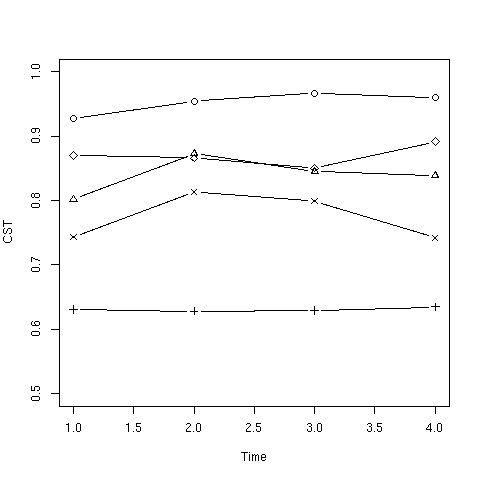
\includegraphics[width=1.0\textwidth]{cst.png}
  \caption{Plot of Flock means for each of the four repeat CST readings in time series order.}
  \label{fig:cst}
\end{figure}

%\end{document}


We see that there is no obvious trend with time. One compression does not influence the results from subsequent compressions. It is therefore satisfactory to use CSTmean.

The correlations between successive readings are shown in Table~\ref{tab:cstrpty}.
% latex table generated in R 3.4.2 by xtable 1.8-2 package
% Thu Nov 30 21:32:31 2017
\begin{table}[ht]
\centering
\label{tab:cstrpty}
\caption{Correlations between the four repeat CST measurements}
\vspace{0.1in}
\begin{tabular}{|r|rrrr|}
  \hline
 & CST1 & CST2 & CST3 & CST4 \\ 
  \hline
CST1 & 1.00 & 0.85 & 0.84 & 0.85 \\ 
  CST2 & 0.85 & 1.00 & 0.86 & 0.87 \\ 
  CST3 & 0.84 & 0.86 & 1.00 & 0.85 \\ 
  CST4 & 0.85 & 0.87 & 0.85 & 1.00 \\ 
   \hline
\end{tabular}
\end{table}


We see that the readings are higly repeatable, and that the repeatability does not decline with time gap.


\subsection{SkinType and collagen}
The collagen measurements for the four SkinTypes will tell us  whether wrinkle and skin looseness are associated with amount and type of collagen.  Figure~\ref{fig:TSTskintype} shows the TST of the four SkinTypes as a boxplot.
%\documentclass{article}
%\usepackage{graphicx,subfigure}
%\begin{document}

\begin{figure}[!h]
  \centering
  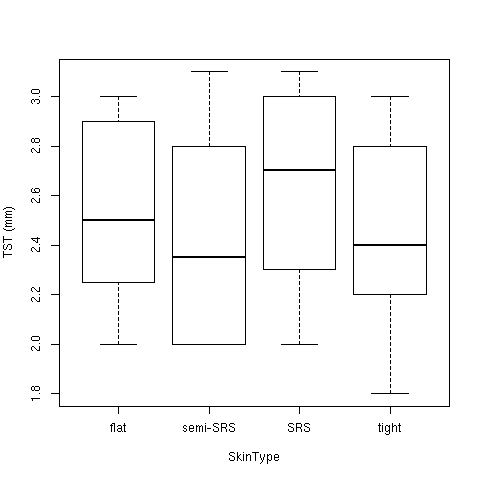
\includegraphics[width=1.0\textwidth]{TSTskintype.png}
  \caption{Boxplot of TST values for all sheep in each of the four SkinTypes}
  \label{fig:TSTskintype}
\end{figure}

%\end{document}


Only the SRS SkinType seems to differ, but we need to test the significance. WE do this with an analysis of variance. Table~\ref{tab:tstaov} shows that there are significant Flock differences, but no significant differences between SkinTypes, and no interaction.
% latex table generated in R 3.4.2 by xtable 1.8-2 package
% Fri Dec  1 20:48:57 2017
\begin{table}[ht]
\caption{Analysis of variance of TST measurements}
\label{tab:tstaov}
\centering
\begin{tabular}{lrrrrr}
  \hline
 & Df & Sum Sq & Mean Sq & F value & Pr($>$F) \\ 
  \hline
Flock          & 4 & 1.53 & 0.38 & 3.13 & 0.0182 \\ 
  SkinType       & 3 & 0.30 & 0.10 & 0.83 & 0.4826 \\ 
  Flock:SkinType & 5 & 0.68 & 0.14 & 1.11 & 0.3617 \\ 
  Residuals      & 93 & 11.36 & 0.12 &  &  \\ 
   \hline
\end{tabular}
\end{table}


So we conclude that the total thickness of collagen in the dermis is not related to either wrinkle (the {\em tight} grade) or to looseness (the {\em SRS and senmi-SRS} grades).

Figure~\ref{fig:CSTskintype} shows the CST of the four SkinTypes as a boxplot.
%\documentclass{article}
%\usepackage{graphicx,subfigure}
%\begin{document}

\begin{figure}[!h]
  \centering
  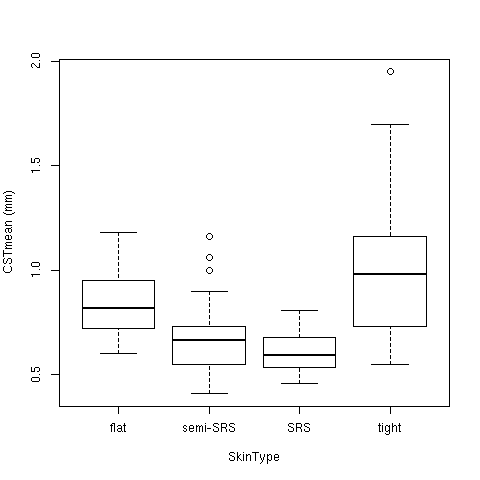
\includegraphics[width=1.0\textwidth]{CSTskintype.png}
  \caption{Boxplot of CST values for all sheep in each of the four SkinTypes}
  \label{fig:CSTskintype}
\end{figure}

%\end{document}


Here we see that there substantial differences, and in the order expected. The {\em tight} SkinType has the greates compressed skin thickness, followed by the {\em flat} SkinType, followed by {\em semi-SRS}, and {\em SRS} SkinType has the smallest CST. We check that this is significant with another analysis of variance in Table~\ref{tab:cstaov}
% latex table generated in R 3.4.2 by xtable 1.8-2 package
% Fri Dec  1 21:12:35 2017
\begin{table}[ht]
\centering
\caption{Analysis of variance of CST measurements}
\label{tab:cstaov}
\begin{tabular}{lrrrrr}
  \hline
 & Df & Sum Sq & Mean Sq & F value & Pr($>$F) \\ 
  \hline
Flock          & 4 & 1.42 & 0.36 & 7.83 & 0.0000 \\ 
  SkinType       & 3 & 0.87 & 0.29 & 6.36 & 0.0006 \\ 
  Flock:SkinType & 5 & 0.26 & 0.05 & 1.14 & 0.3434 \\ 
  Residuals      & 93 & 4.22 & 0.05 &  &  \\ 
   \hline
\end{tabular}
\end{table}

  
In this case both the Flock and SkinType effects are significant, but not the interaction. So we conclude that thickness of collagen in the dermis after compression is greater in wrinkled sheep ({\em tight} grade), and is reduced in sheep with loose skin ({\em SRS} grade). This agrees with the proposition that the orderly trio groups in {\em SRS} grade sheep are a  consequence of less development of collagen tissue.

We suspect that because the SkinType differences were in CST but not in TST that what we are looking at is differences between hard and soft collagen, the latter being more readily compressed. We can express this more succinctly by analysing compressibility (CMP).

Figure~\ref{fig:CMPskintype} shows the CMP measurement of the four SkinTypes as a boxplot.
%\documentclass{article}
%\usepackage{graphicx,subfigure}
%\begin{document}

\begin{figure}[!h]
  \centering
  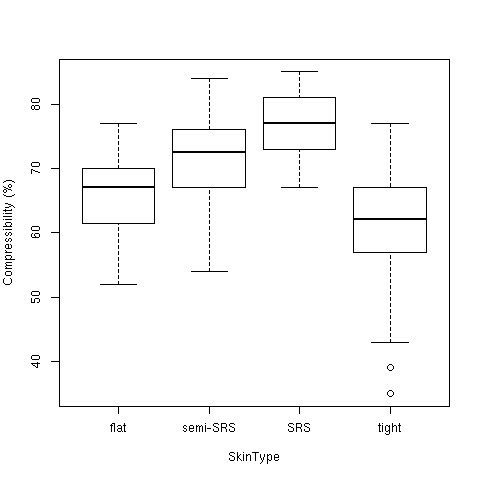
\includegraphics[width=1.0\textwidth]{CMPskintype.png}
  \caption{Boxplot of CMP values for all sheep in each of the four SkinTypes}
  \label{fig:CMPskintype}
\end{figure}

%\end{document}


Here we see a similar picture to the CST graphs, there being substantial differences and in the order expected. The {\em tight} grade, which is wrinkles, is only 60 percent compressible, and the others range up to 80 percent in order. We check the significvance in another analysis of variance in Table~\ref{tab:cmpaov}
tex table generated in R 3.4.2 by xtable 1.8-2 package
% Fri Dec  1 21:33:14 2017
\begin{table}[ht]
\centering
\caption{Analysis of variance of skin compressibility (CMP) measurements}
\label{tab:cmpaov}
\begin{tabular}{lrrrrr}
  \hline
 & Df & Sum Sq & Mean Sq & F value & Pr($>$F) \\ 
  \hline
Flock          & 4 & 2986.36 & 746.59 & 15.72 & 0.0000 \\ 
  SkinType       & 3 & 1172.83 & 390.94 & 8.23 & 0.0001 \\ 
  Flock:SkinType & 5 & 436.47 & 87.29 & 1.84 & 0.1131 \\ 
  Residuals      & 93 & 4417.96 & 47.50 &  &  \\ 
   \hline
\end{tabular}
\end{table}


As for CST the Flock and SkinType effects are significant, but not the interaction. So we conclude that compressibility is least in wrinkled sheep ({\em tight} grade), and is greatest in sheep with loose skin ({\em SRS} grade). So the collagen is harder in wrinkled sheep, and softer in sheep with loose skin. This also agrees with the proposition that the orderly trio groups in {\em SRS} grade sheep are a  consequence of less development of collagen tissue.

\subsection{Collagen Flock differences}
\label{sec:collflock}
A feature of the analyses of the previous section is that there were  large and significant Flock differences in all three traits (TST, CSTmean, and CMP). We documented  these in Table~\ref{tab:collmeans}. It should be noted that not all SkinTypes were present in each Flock, so there could be some bias in these Flock means.  We can circumvent this to some extent by looking at the two-way table of means Flock x SkinType. We do this for CMP in Table~\ref{tab:fxst}
\begin{table}[ht]
\centering
\label{tab:fxst}
\caption{Means of CST for all combinations of Flock and SkinType. The NA entries are cells with no data available.}
\vspace{0.1in}
\begin{tabular}{|r|rrrr|}
  \hline
Flock & tight & flat & semi-SRS  & SRS \\ 
  \hline
1 & 55.2 & 64.32 & NA & NA  \\
2 & 53.0 & NA & 66.3 & 72.3 \\
3 &  NA & NA & 75.0 & 78.1 \\
4 & 67.3 & 69.7 & 69.0 & NA \\
5 & 63.0 & NA & 65.8 & 75.0 \\
   \hline
\end{tabular}
\end{table}


We see that the SkinType differences are consistent across Flocks. We also see that the Flock differences are consistent across SkinTypes. That is what the absence of interaction in Table~\ref{tab:cmpaov} shows. 

So we need to reach an understanding that SkinType is not the only thing correlated with collagen measurements. Flocks difffer in TST, CSTmean and CMP in ways that are not explained by Flock differences in the proportions of sheep with each SkinType (look for example at the semi-SRS column of Table\ref{tab:fxst}). These SkinType independent Flock differences may be genetic or non-genetic. Something else affects the amount and hardness of collagen without affecting SkinType. We are sure of one thing, it is not a shift in classing standards for SkinType between Flocks.

\subsection{Collagen and skin softness appraisal}
We have another way of checking on whether the CSTmean and CMP measurements actually represeent collagen softness. We can compare them with the SkinSoft scores.
The correlations between SkinSoft score and the 3 collagen measurements are given in Table~\ref{tab:corsoft}
% latex table generated in R 3.4.2 by xtable 1.8-2 package
% Sat Dec  2 21:20:13 2017
\begin{table}[ht]
\centering
\caption{Correlations among TST, CSTmean, CMP, and SkinSoft score}
\label{tab:corsoft}
\begin{tabular}{rrrrr}
  \hline
 & TST & CSTmean & CMP & SkinSoftScore \\ 
  \hline
TST & 1.00 & 0.33 & 0.14 & -0.29 \\ 
  CSTmean & 0.33 & 1.00 & -0.88 & -0.72 \\ 
  CMP & 0.14 & -0.88 & 1.00 & 0.61 \\ 
  SkinSoftScore & -0.29 & -0.72 & 0.61 & 1.00 \\ 
   \hline
\end{tabular}
\end{table}


The correlation of SkinSoft score with CSTmean is slightly higher than that with CMP. Dividing by TST may be introducing errors. There is only a small correlation with TST, and that is expected. Bending softness is more a matter of softness of the material than of minor variations in material thickness. Compare sheet aluminium with sheet steel, minor thickness variations will not make sheet steel bend like aluminium.

\subsection{Collagen and follicle characteristics}
\subsubsection{S/P ratio}
 Figure~\ref{fig:sptst} shows the correlation beetween S/P ratio and TST measurements across all Flocks.
%\documentclass{article}
%\usepackage{graphicx,subfigure}
%\begin{document}

\begin{figure}[!h]
  \centering
  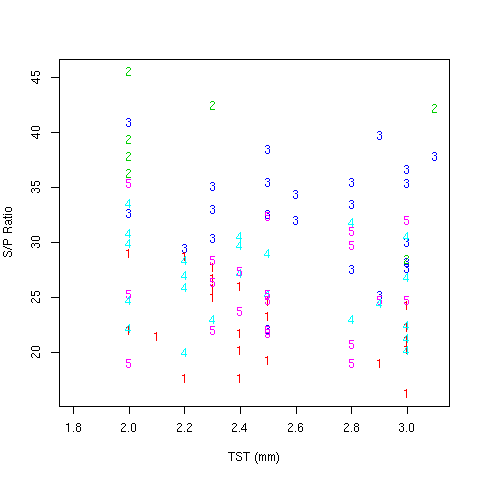
\includegraphics[width=1.0\textwidth]{sptst.png}
  \caption{Plot of TST measurements against S/P ratio. The numbered points reveal the Flock to which each data point belongs. The correlation of these points is 0.11 which is not significant for 106 observations}
  \label{fig:sptst}
\end{figure}

%\end{document}


The correlation of 0.11 is not significant.

 Figure~\ref{fig:spcst} shows the correlation between S/P ratio and CSTmean measurements across all Flocks.
%\documentclass{article}
%\usepackage{graphicx,subfigure}
%\begin{document}

\begin{figure}[!h]
  \centering
  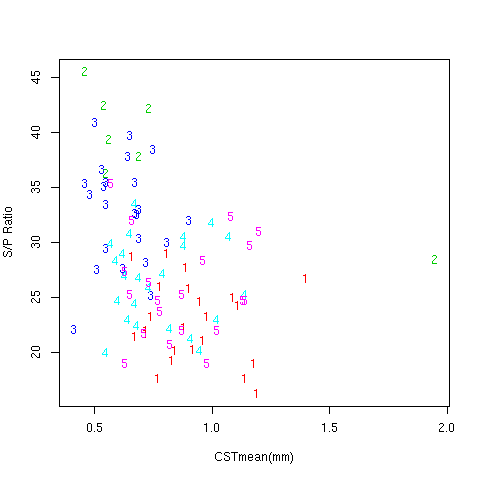
\includegraphics[width=1.0\textwidth]{spcst.png}
  \caption{Plot of CSTmean measurements against S/P ratio. The numbered points reveal the Flock to which each data point belongs. The correlation of these points is -0.38 which is significant at the 1 percent level for 106 observations}
  \label{fig:spcst}
\end{figure}

%\end{document}


The correlation 0f -0.38 is significant $(P<.01)$. There is one serious outlier point in Figure~\ref{fig:spcst} - the green point from Flock 2 at the right of the Figure. It was a sheep with an extremely thick tight skin, but it did not have an unusually low S/P ratio. If we omit this one outlier the correlation becomes -0.44 which is also significant $(P<.01)$.

The other thing to note in Figure~\ref{fig:spcst} is that the Flocks tend to form a series of groups along the curve. That is there is  also a negative relationship between the Flock means, in addition to that among individual values. 
If we plot the same points but label each point with its SkinType, we get Figure~\ref{fig:spcstskin}
%\documentclass{article}
%\usepackage{graphicx,subfigure}
%\begin{document}

\begin{figure}[!h]
  \centering
  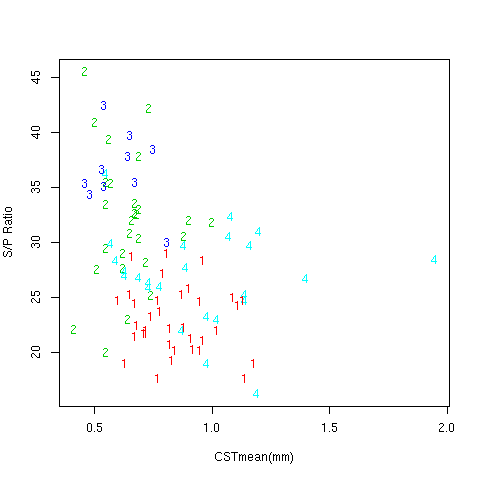
\includegraphics[width=1.0\textwidth]{spcstskin.png}
  \caption{Plot of CSTmean measurements against S/P ratio. The numbered points reveal the SkinType to which each data point belongs (1="flat", 2="semi-SRS", 3="SRS", 4="tight"). The correlation of these points is -0.38 which is significant at the 1 percent level for 106 observations}
  \label{fig:spcstskin}
\end{figure}

%\end{document}


This shows that the four SkinTypes also form a series of groups so there is also a negative relationship between SkinType means. The correlation is of course the same as in Figure~\ref{fig:spcst}.

We noted in section~\ref{sec:collflock} that SkinType differences in CSTmean and Flock differences in CSTmean seemed to be independent. However now we observe that so far as the correlation of CSTmean with S/P ratio is concerned, SkinType differences, and Flock differences and individual differences all seem to part of the same continuous negative relationship. This is something of a mystery. What it says is that it doesnt matter whether differences in CSTmean are observable as SkinType or not, they are all correlated with S/P ratio. Perhaps the SkinType classing grades are not observing some of the collagen differences.

The main point is that there is a significant negative relationship of CSTmean with S/P ratio. This is what the collagen-link hypothesis predicts, so it is an important confirmation.

 Figure~\ref{fig:spcmp} shows the correlation between S/P ratio and CMP measurements across all Flocks.
%\documentclass{article}
%\usepackage{graphicx,subfigure}
%\begin{document}

\begin{figure}[!h]
  \centering
  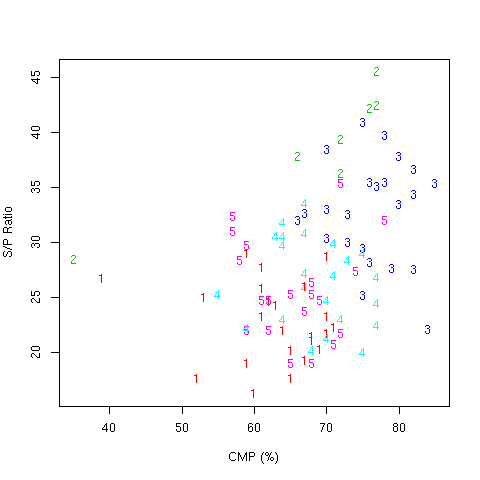
\includegraphics[width=1.0\textwidth]{spcmp.png}
  \caption{Plot of CMP measurements against S/P ratio. The numbered points reveal the Flock to which each data point belongs. The correlation of these points is 0.36 which is significant at the 1 percent level for 106 observations}
  \label{fig:spcmp}
\end{figure}

%\end{document}


For compressibility versus S/P ratio there are two outlier points, and the correlation (0.36) is similar to that for CSTmean, but of course is now positive - soft compressible skins have a high S/P ratio. Again the remarks about Flocks grouping along the relationship line apply. We do not bother to look at a graph showing SkinType instead of Flock for each point, because the same should apply as for CSTmean, above.

\subsubsection{Follicle number per unit area}
We have chosen to look at S/P ratio rather than follicle number per unit area. There are two reasons
\begin{itemize}
\item it is the secondary follicle number which the collagen-link hypothesis predicts would be affected by excess collagen formation. Follicle number per unit area would of course reflect this, but it is a more indirect consequence
\item S/P ratio is basically a way of expressing secondary follicle density independent of any effects of varying body growth on skin expansion. So we would expect S/P ratio to be free of some other confounding factors
\end{itemize}

What we shall do is just have a quick look at follicle number by computing correlations. These are shown in Table~\ref{tab:collfollcor}. We also include the SkinSoft score here, as it gives similar results to the collagen softness measurements.
% latex table generated in R 3.4.2 by xtable 1.8-2 package
% Mon Dec  4 21:12:12 2017
\begin{table}[ht]
\centering
\caption{Correlations among TST, CSTmean, CMP, SkinSoft, S/P, and Fn}
\label{tab:collfollcor}
\begin{tabular}{|rrrrrrr|}
  \hline
 & TST & CSTmean & CMP & SkinSoft & S/P & Fn \\ 
  \hline
TST & 1.00 & 0.34 & 0.13 & -0.26 & -0.11 & 0.19 \\ 
  CSTmean & 0.34 & 1.00 & -0.88 & -0.73 & -0.37 & -0.33 \\ 
  CMP & 0.13 & -0.88 & 1.00 & 0.64 & 0.36 & 0.43 \\ 
  SkinSoft & -0.26 & -0.73 & 0.64 & 1.00 & 0.36 & 0.26 \\ 
  S/P & -0.11 & -0.37 & 0.36 & 0.36 & 1.00 & 0.38 \\ 
  Fn & 0.19 & -0.33 & 0.43 & 0.26 & 0.38 & 1.00 \\ 
   \hline
\end{tabular}
\end{table}


As expected, follicle number has the same relationship with CSTmean and CMP as does S/P ratio. It has a different correlation with TST, but these correlations ( -0.11 and 0.19) are small and the 0.19 is only just significant at the $(P,.05)$ level. The surprise is that the correlation of SkinSoft score with S/P ratio is as strong as the correlations of the CSTmean and CMP measrements with S/P ratio. The scoring is clearly just as accurate as the measurements. It does however have a different lower correlation with Fn. 

This proves that we can put follicle number aside and just concentrate on the relationships of collagen with S/P ratio.


\subsection{Collagen and Fibre growth}
\subsubsection{Mean secondary fibre diameter}
The collagen-link hypothesis postulates that sheep with high and/or hard collagen skins will have higher average diameter of secondary fibres, more curved fibres, and a lower fibre length growth rate. It  also suggests that sheep with high and/or hard collagen skins will have a high follicle unevenness score , which we know to be associated with high variability of fibre diameter. The effect on mean secondary fibre diameter is not direct, it is secondary to the effect on S/P ratio, it being known that highly branched follicles grow finer fibres.

Figure~\ref{fig:tstds} shows the correlation of TST measurement with meandiameter of secondary fibres.
%\documentclass{article}
%\usepackage{graphicx,subfigure}
%\begin{document}

\begin{figure}[!h]
  \centering
  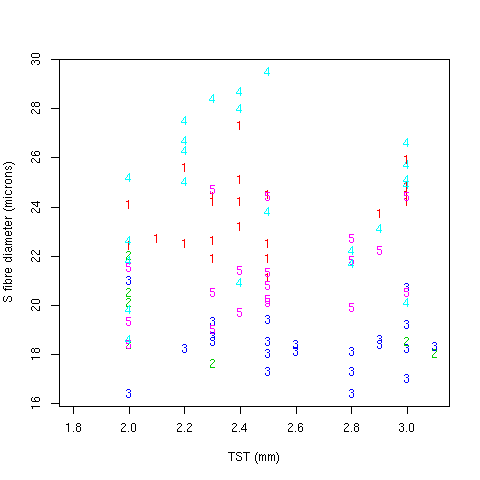
\includegraphics[width=1.0\textwidth]{tstds.png}
  \caption{Plot of TST measurements against mean secondary fibre diameter. The numbered points reveal the Flock to which each data point belongs. The correlation of these points is -0.04 which is not significant for 106 observations}
  \label{fig:tstds}
\end{figure}

%\end{document}


The correlation is close to zero and not significant. 

Figure~\ref{fig:cstds} shows the correlation of CSTmean measurement with mean diameter of secondary fibres.
%\documentclass{article}
%\usepackage{graphicx,subfigure}
%\begin{document}

\begin{figure}[!h]
  \centering
  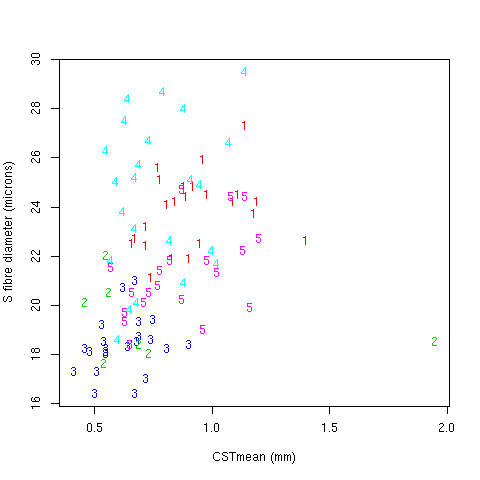
\includegraphics[width=1.0\textwidth]{cstds.png}
  \caption{Plot of CSTmean measurements against mean secondary fibre diameter. The numbered points reveal the Flock to which each data point belongs. The correlation of these points is 0.34 which is significant at the 1 percent level for 106 observations}
  \label{fig:cstds}
\end{figure}

%\end{document}


This correlation is 0.34 and is significant $(P<0.01)$. Flock 4 seems to have a higher mean S diameter than the other flocks, but this difference is not associated with a correlated difference in CSTmean. Hence Flock 4 appears above the other points on the graph. We know there things other than CSTmean which affect mean S fibre diameter - for example the numbers of pre-poapilla cells which initiate the secondary follicle.  There is one outlier point.

Figure~\ref{fig:cmpds} shows the correlation of CMP measurement with mean diameter of secondary fibres.
%\documentclass{article}
%\usepackage{graphicx,subfigure}
%\begin{document}

\begin{figure}[!h]
  \centering
  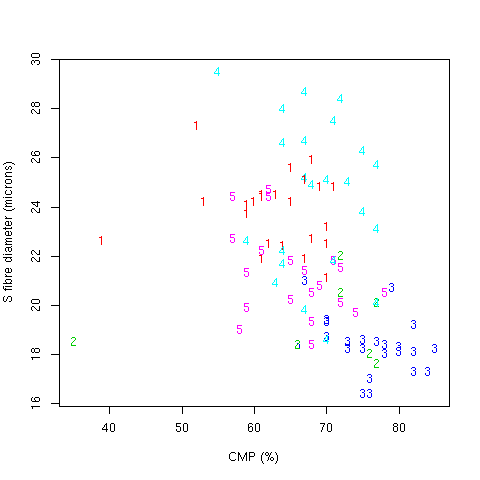
\includegraphics[width=1.0\textwidth]{cmpds.png}
  \caption{Plot of CMP measurements against mean secondary fibre diameter. The numbered points reveal the Flock to which each data point belongs. The correlation of these points is -0.40 which is significant at the 1 percent level for 106 observations}
  \label{fig:cmpds}
\end{figure}

%\end{document}


This correlation is -0.40 and is significant $(P<0.01)$. Again Flock 4 seems to have a higher mean S diameter than the other flocks, and appears above the other points on the graph. There are two outlier points.

\subsubsection{Standard deviation of secondary fibre diameter}
Figure~\ref{fig:tstdssd} shows the correlation of TST measurement with standard deviation of diameter of secondary fibres.
%\documentclass{article}
%\usepackage{graphicx,subfigure}
%\begin{document}

\begin{figure}[!h]
  \centering
  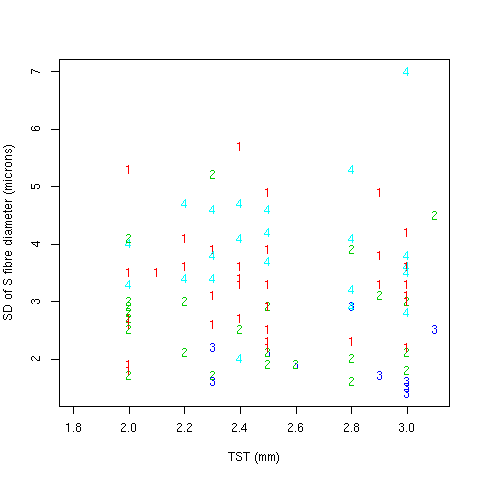
\includegraphics[width=1.0\textwidth]{tstdssd.png}
  \caption{Plot of TST measurements against standard deviation of secondary fibre diameter. The numbered points reveal the Flock to which each data point belongs. The correlation of these points is -0.01 which is not significant for 106 observations}
  \label{fig:tstdssd}
\end{figure}

%\end{document}


The correlation is close to zero and not significant.

Figure~\ref{fig:cstdssd} shows the correlation of CSTmean measurement with standard deviation of diameter of secondary fibres.
%\documentclass{article}
%\usepackage{graphicx,subfigure}
%\begin{document}

\begin{figure}[!h]
  \centering
  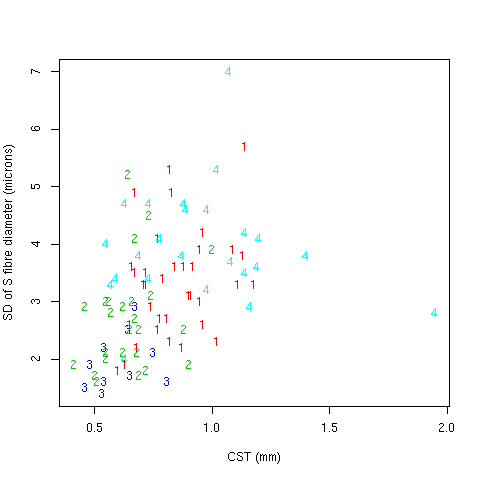
\includegraphics[width=1.0\textwidth]{cstdssd.png}
  \caption{Plot of CST measurements against standard deviation of secondary fibre diameter. The numbered points reveal the SkinType to which each data point belongs. The correlation of these points is 0.39 which is significant at the 1 percent level for 106 observations}
  \label{fig:cstdssd}
\end{figure}

%\end{document}


The correlation is 0.39 and is significant $(P<0.01)$. In this case there is again suggestion of Flock 4 being higher in DsSD than expected from CSTmean. So in this case other factors are also operating. The effect of collagen on DsSD may be via mean Ds, or may be via the {\em  hard collagen - curved follicles - curved fibres link}. It is known that skins with high follicle curvature score also have high follicle unevenness score (genetic correlation is $0.82\pm0.02$ Jackson(2017)~\cite{jack:17a}), and therefore grow fibres of less uniform diameter.

Figure~\ref{fig:cmpdssd} shows the correlation of CMP measurement with standard deviation of diameter of secondary fibres.
%\documentclass{article}
%\usepackage{graphicx,subfigure}
%\begin{document}

\begin{figure}[!h]
  \centering
  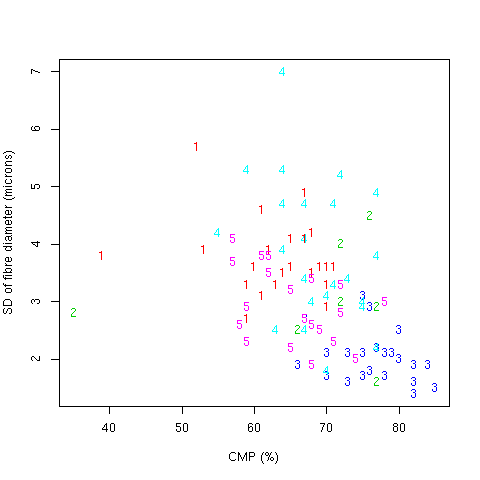
\includegraphics[width=1.0\textwidth]{cmpdssd.png}
  \caption{Plot of CMP measurements against standard deviation of secondary fibre diameter. The numbered points reveal the Flock to which each data point belongs. The correlation of these points is -0.43 which is significant at the 1 percent level for 106 observations}
  \label{fig:cmpdssd}
\end{figure}

%\end{document}


The correlation is -0.43 and is significant $(P<0.01)$.  Again Flock 4 stands out, so the remarks above apply. Hard collagen makes curved follicles, which are uneven in their anatomy and in their fibre growth. 

\subsubsection{Follicle and fibre curvature}
It is known that follicle curvature and intrinsic fibre curvature are very closely related, and probably are exactly the same thing. The following results for follivcle curvarure should also therefore apply to fibre curvature.

Correlation of TST with Follicle curvature was low ( 0.118 and not significant). The graph is not reported here.

Figure~\ref{fig:CSTFc} shows the correlation of CSTmean measurement with follicle curvature. 
%\documentclass{article}
%\usepackage{graphicx,subfigure}
%\begin{document}

\begin{figure}[!h]
  \centering
  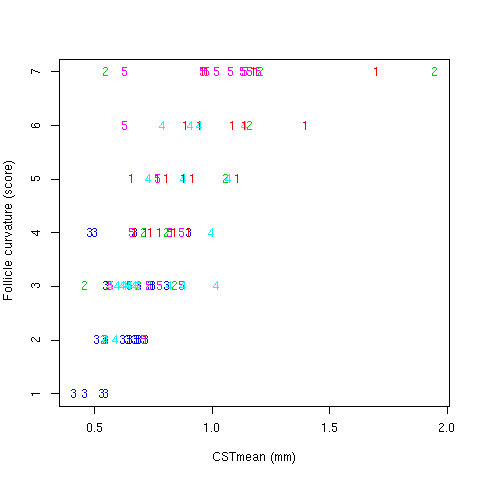
\includegraphics[width=1.0\textwidth]{CSTFc.png}
  \caption{Plot of CSTmean measurements against follicle curvature score. The numbered points reveal the Flock to which each data point belongs. The correlation of these points is 0.72 which is significant at the 1 percent level for 106 observations}
  \label{fig:CSTFc}
\end{figure}

%\end{document}


The correlation is  0.719 and is significant $(P<0.01)$. Note the triangular shape of the scatter of points; it implies that a low CST can be any follicle curvature score from 1 to 7, while a high CST can only be follicle curvature score 6 or 7. So alot of hard collagen constrains the follicles to being curved, but the follicles are free to do anything if the collagen is little or soft. That implies that there might be two factors affecting curvture - a 'natural' curvature of the follicles, and and overriding constraint added by the collagen. 

The correlation of CMP with follicle curvature is shown in in Figure~\ref{fig:CMPFc}
%\documentclass{article}
%\usepackage{graphicx,subfigure}
%\begin{document}

\begin{figure}[!h]
  \centering
  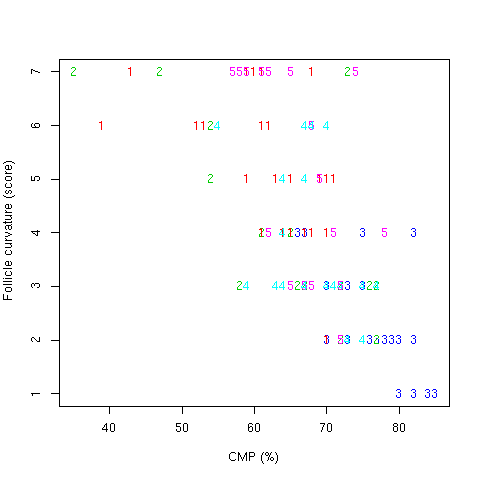
\includegraphics[width=1.0\textwidth]{CMPFc.png}
  \caption{Plot of CMP percentages against follicle curvature score. The numbered points reveal the Flock to which each data point belongs. The correlation of these points is -0.69 which is significant at the 1 percent level for 106 observations}
  \label{fig:CMPFc}
\end{figure}

%\end{document}


This correlation is -0.69 and is significant $(P<0.01)$. The correlation is similat to that between follicle curvature and CSTmean, but with opposite sign, and the triangular scatter of points is still present. 

We need to try and get some insight into what sort of sheep are falling into the top corner of the triange in Figures ~\ref{fig:CSTFc} and ~\ref{fig:CMPFc}. They do not belong to any particular flock, and on redrawing the above fgraphs showing SkinType of each point , we saw that they do not belong to any particular SkinType. The only association we could find is a suggestion that points toward the corner of the triangle have a low standard deviation of secondary fibre diameter. This is shown in Figure~\ref{fig:CSTFcbyDsSD}
%\documentclass{article}
%\usepackage{graphicx,subfigure}
%\begin{document}

\begin{figure}[!h]
  \centering
  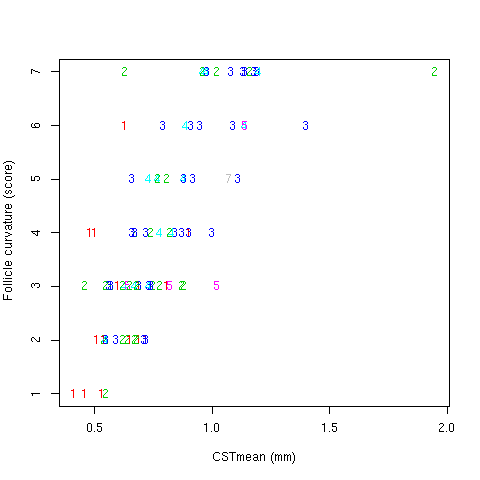
\includegraphics[width=1.0\textwidth]{CSTFcbyDsSD.png}
  \caption{Plot of CSTmean measurements against follicle curvature score. The numbered points reveal the standard deviation of secondary fibre diameter to which each data point belongs. The correlation of these points is 0.72 which is significant at the 1 percent level for 106 observations}
  \label{fig:CSTFcbyDsSD}
\end{figure}

%\end{document}


This is not entirely convincing. It needs further investigation, probably with a wider range of data.

\subsubsection{Follicle unevenness}
It is known that follicle unevenness score and standard deviation of fibre diameter are correlated. The follicle results should therefore be similar to those for DsSD above.

Correlation of TST with Follicle unevenness was low ( 0.162 and not significant). The graph is not reported here.

Figure~\ref{fig:CSTFu} shows the correlation of CSTmean measurement with follicle unevenness score.
%\documentclass{article}
%\usepackage{graphicx,subfigure}
%\begin{document}

\begin{figure}[!h]
  \centering
  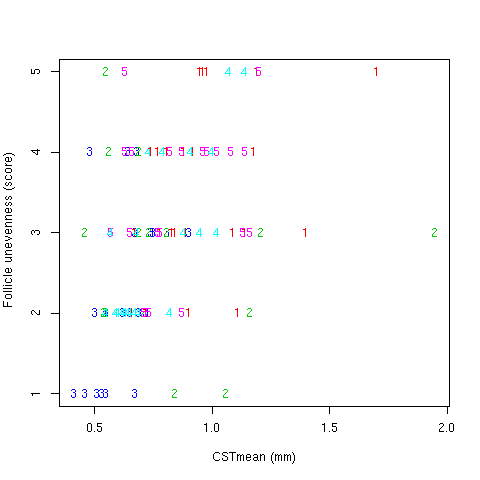
\includegraphics[width=1.0\textwidth]{CSTFu.png}
  \caption{Plot of CSTmean measurements against follicle unevenness score. The numbered points reveal the Flock to which each data point belongs. The correlation of these points is 0.72 which is significant at the 1 percent level for 106 observations}
  \label{fig:CSTFu}
\end{figure}

%\end{document}


This correlation is 0.41 and is significant $(P<0.01)$. Again we see thhe triangular scatter of points. A high CST means highly uneven follicles, but a low CST can be anything.

Figure~\ref{fig:CMPFu} shows the correlation of CMP percentage with follicle unevenness score.
%\documentclass{article}
%\usepackage{graphicx,subfigure}
%\begin{document}

\begin{figure}[!h]
  \centering
  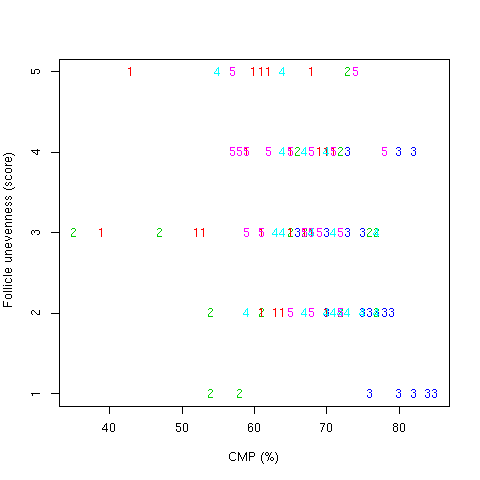
\includegraphics[width=1.0\textwidth]{CMPFu.png}
  \caption{Plot of CMP percentages against follicle unevenness score. The numbered points reveal the Flock to which each data point belongs. The correlation of these points is -0.34 which is significant at the 1 percent level for 106 observations}
  \label{fig:CMPFu}
\end{figure}

%\end{document}


This correlation is 0.41 and is significant $(P<0.01)$. Again we see thhe triangular scatter of points. A high CMP means highly uneven follicles, but a low CST can be anything.


\subsubsection{Follicle depth}
We do not expect any relationship between collagen measurements and follicle depth, except perhaps with TST.

Figure~\ref{fig:TSTFd} shows the correlation of follicle depth with TST.
%\documentclass{article}
%\usepackage{graphicx,subfigure}
%\begin{document}

\begin{figure}[!h]
  \centering
  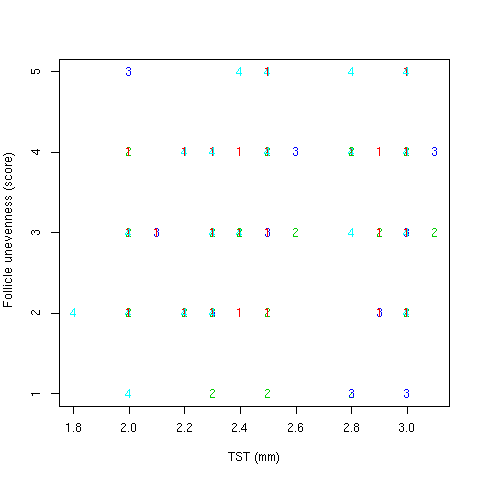
\includegraphics[width=1.0\textwidth]{TSTFu.png}
  \caption{Plot of TST percentages against follicle depth measurement. The numbered points reveal the Flock to which each data point belongs. The correlation of these points is 0.30 which is significant at the 1 percent level for 106 observations}
  \label{fig:TSTFd}
\end{figure}

%\end{document}


This correlation is 0.30 and is significant $(P<0.01)$.

The correlations of follicle depth with CSTmean and CMP were small ( 0.23 and -0.11 respectively). THese are not shown as scatterplots.

\subsubsection{Fibre length growth rate}
We do not have fibre length growth rate data in this dataset.  The best we can do is to look elsewhere for the relationship between follicle curvature and fibre length growth rate.  We have a dataset consisting of 306 sheep from 12 flocks, for which follicle curvature and mean fibre length growth rate were measured.  These data are plotted in Figure~\ref{fig:fcfl}
%\documentclass{article}
%\usepackage{graphicx,subfigure}
%\begin{document}

\begin{figure}[!h]
  \centering
  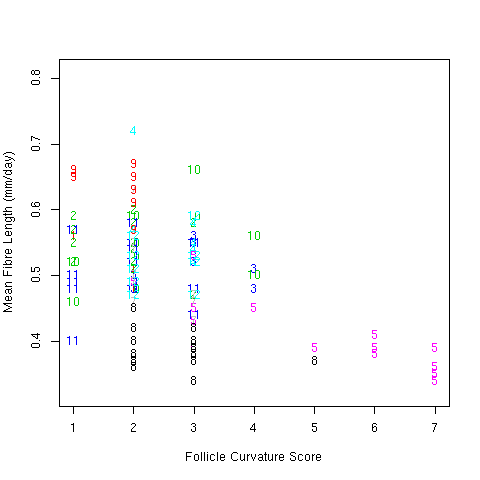
\includegraphics[width=1.0\textwidth]{fcfl.png}
  \caption{Plot of follicle curvature score against mean fibre length growth rate (mm/day). The numbered points reveal the Flock to which each data point belongs.The correlation of these points is -0.52 which is significant at the 1 percent level for 106 observations}
  \label{fig:fcfl}
\end{figure}

%\end{document}


Again we get the familiar triangular scatter of points. High follicle curvature sheep only have low fibre length growth rates, but low follicle curvature sheep can have any fibre length growth rate over the full range from 0.4 to 0.8 mm/day. The correlation is -0.52 ( significant $P<0.01$) but this is not very meaningful because of the peculiar scatter of the points. The coloured numbers representing each point identify which of the 12 flocks each sheep came from.

So if follicle curvature indicates presence of lots of collagen, then fibre length growth rate is reduced in the presence of lots of collagen, but can be anything in the presence of low levels of collagen.


\subsubsection{Summary of collagen measures and fibre properties}


We will summarize what we have on collagen and fibre properties as a table of correlations (Table~\ref{tab:collfibcor}).
% latex table generated in R 3.4.2 by xtable 1.8-2 package
% Sat Jan 20 21:08:18 2018
\begin{center}
\begin{landscape}
\begin{table}[ht]
\caption{Correlations amongTST, CSTmean, CMP, SkinSoft, Ds, DsSD, Fc, Fu, and Fd} 
\vspace{0.2in}
\label{tab:collfibcor}
\begin{tabular}{|rrrrrrrrrr|}
  \hline
 & TST & CSTmean & CompressPer & SkinSoftScore & Ds & DsSD & Fc & Fu & Fdmean \\ 
  \hline
TST & 1.00 & 0.34 & 0.13 & -0.26 & -0.04 & -0.01 & 0.13 & 0.13 & 0.28 \\ 
  CSTmean & 0.34 & 1.00 & -0.88 & -0.73 & 0.34 & 0.39 & 0.74 & 0.47 & 0.26 \\ 
  CompressPer & 0.13 & -0.88 & 1.00 & 0.64 & -0.40 & -0.43 & -0.71 & -0.42 & -0.16 \\ 
  SkinSoftScore & -0.26 & -0.73 & 0.64 & 1.00 & -0.29 & -0.29 & -0.68 & -0.44 & -0.23 \\ 
  Ds & -0.04 & 0.34 & -0.40 & -0.29 & 1.00 & 0.73 & 0.45 & 0.35 & 0.26 \\ 
  DsSD & -0.01 & 0.39 & -0.43 & -0.29 & 0.73 & 1.00 & 0.36 & 0.31 & 0.35 \\ 
  Fc & 0.13 & 0.74 & -0.71 & -0.68 & 0.45 & 0.36 & 1.00 & 0.71 & 0.14 \\ 
  Fu & 0.13 & 0.47 & -0.42 & -0.44 & 0.35 & 0.31 & 0.71 & 1.00 & 0.12 \\ 
  Fdmean & 0.28 & 0.26 & -0.16 & -0.23 & 0.26 & 0.35 & 0.14 & 0.12 & 1.00 \\ 
   \hline
\end{tabular}
\end{table}
\end{landscape}
\end{center}



The SkinSoft score shows basically the same correlations as CMP, and the same with opposite sign as CSTmean. CSTmean and CMP have similar correlations with fibre properties.

\subsection{Will variations in amount of follicle tissue affect CST measurement?}
The skin specimen which is being compressed in CST measurement contains tissues other than collagen. So it is possible that variations in these other tissues affect compressed thickness. In particular, follicle tissue is likely to be much less compressible than collagen. To investigate this we need a measure of the amount of follicle tissue per unit area or per unit volume of skin. 

We start by noting that the diameter of a follicle stem at sebacious gland level is close to 3 times the diameter of the fibre it contains. So the area of follicle tissue per $mm^{2}$ at that level is
\begin{displaymath}
F_{a} = 10^{-6} F_{n} \pi \left[\frac{3D}{2}\right]^{2}
\end{displaymath}
$F_{a}$ will vary between 0 and 1 and will represent the follicle tissue area in $mm^{2}$ per $mm^{2}$, so it is unitless. 

We next note that the average length of follicles is represented by follicle depth (Fd) in $mm$.  So the volume of follicle tissue per $mm^{2}$  of cross section is 
\begin{displaymath}
F_{v} = F_{a} Fd
\end{displaymath}
$F_{v}$ will be $mm^{3}$ of follicle tissue per $mm^{2}$ of cross section, so it will be in $mm$. 

Now we want to see whether either $F_{a}$ or $F_{v}$ varies with CST. So we do a regression of CST on Age and either $F_{a}$ or $F_{v}$ . Neither of these regressions were significant. This is shown in the analyses of variance given in Tables~\ref{tab:cstfa} and ~\ref{tab:cstfv}
% latex table generated in R 3.4.2 by xtable 1.8-2 package
% Wed Jan 24 20:56:38 2018
\begin{table}[ht]
\centering
\caption{Analysis of variance of regression of CSTmean on Age, Fa, and Fdmean}
\label{tab:cstfa}
\begin{tabular}{lrrrrr}
  \hline
 & Df & Sum Sq & Mean Sq & F value & Pr($>$F) \\ 
  \hline
Age         & 1 & 0.20 & 0.20 & 3.74 & 0.0563 \\ 
  Fa          & 1 & 0.00 & 0.00 & 0.03 & 0.8623 \\ 
  Fdmean      & 1 & 0.28 & 0.28 & 5.29 & 0.0237 \\ 
  Residuals   & 92 & 4.90 & 0.05 &  &  \\ 
   \hline
\end{tabular}
\end{table}


% latex table generated in R 3.4.2 by xtable 1.8-2 package
% Wed Jan 24 20:59:47 2018
\begin{table}[ht]
\centering
\caption{Analysis of variance of regression of CSTmean on Age and Fv}
\label{tab:cstfv}
\begin{tabular}{rrrrr}
  \hline
 & Estimate & Std. Error & t value & Pr($>$$|$t$|$) \\ 
  \hline
(Intercept) & 0.6912 & 0.0806 & 8.58 & 0.0000 \\ 
  Fv & 0.2088 & 0.1593 & 1.31 & 0.1930 \\ 
   \hline
\end{tabular}
\end{table}

The Age effect is not significant. In Table~\ref{tab:cstfa}, Fdmean was included in the regression, and it was significant but only at the $P<.05$ level. We looked at the plot of CSTmean against Fdmean; it is a low correlation ( 0.23 ). 
o we re-did the regression just regressing CST on Fd. The result is shown in Table~\ref{tab:cstfd}
% latex table generated in R 3.4.2 by xtable 1.8-2 package
% Wed Jan 24 21:19:42 2018
\begin{table}[ht]
\centering
\caption{Analysis of variance of regression of CSTmean on Fdmean}
\label{tab:cstfd}
\begin{tabular}{lrrrrr}
  \hline
 & Df & Sum Sq & Mean Sq & F value & Pr($>$F) \\ 
  \hline
Fdmean & 1 & 0.36 & 0.36 & 5.97 & 0.0163 \\ 
  Residuals & 103 & 6.28 & 0.06 &  &  \\ 
   \hline
\end{tabular}
\end{table}


The follicle depth regression is now almost significant at $P<0.01$
We proceed to see if adjusting CSTmean for Fd does anything to the relationship of CST with Fc. Figure~\ref{fig:CSTcFdxFc} shows the relationship of follicle depth corrected CST to follcile curvature.
%\documentclass{article}
%\usepackage{graphicx,subfigure}
%\begin{document}

\begin{figure}[!h]
  \centering
  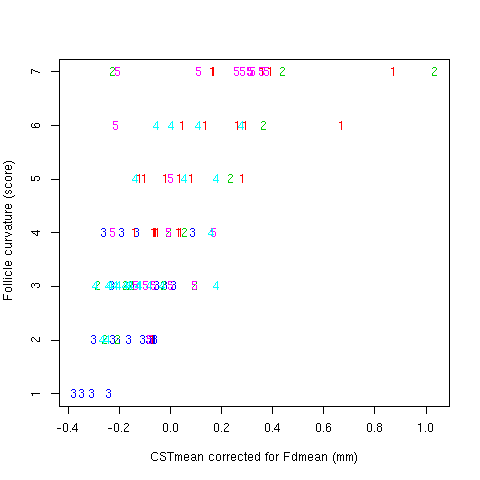
\includegraphics[width=1.0\textwidth]{CSTcFdxFc.png}
  \caption{Plot of CMP measurements corrected for follicle depth against Follicle curvature score . The numbered points reveal the Flock to which each data point belongs. The correlation of these points is 0.71 which is significant at the 1 percent level for 106 observations}
  \label{fig:CSTcFdxFc}
\end{figure}

%\end{document}


The correlation is 0.71. If we compare to CSTmean not corrected for Fd, its correlation with Fc was 0.72. Therefore the correction of CST for Fd did nothing to help with relating CST to Fc. The point scatter is still triangular. We can not explain that phenomenon by correcting CST.


The conclusion is clear. We cannot find any basis for adjustng CST measurements for amount of follicle tissue.


\clearpage
\section{Discussion}
\subsection{Correlations in general}
 All of the correlations we have examined are in the directions expected from the collagen-link hypothesis.  So in that sense, we have no data that would negate the hypothesis. However, that is far from a proof. Correlation does not imply causation, it may imply that the two correlated items have a common cause; in fact this is what we argue, that the collagen measurements and follicle measurements are negatively correlated because fibroblast development and pre-papilla cell development both depend on a shared resource. We think that this shared resource is the population of mesenchymal stem cells which are available for differentiation at the appropriate stage. It may not be that, it could be some protein or biochemical molecule required for differentiation of both cell types.

The correlations all have the expected sign, but they are not large. For example a 0.40 correlation only implies 16 percent of the variance is in common. This is not unexpected for two reasons
\begin{itemize}
\item measurement errors, particularly for the new collagen measurements, will reduce observed correlations
\item factors other than the relationships we are postulating will affect our measurements, diluting the observed relationships. We look at some specific cases of this below.
\end{itemize}

\subsection{Collagen development and pre-papilla cell development}
Negative correlations , if we ignore the trivial case where one variable is measured on an inverse scale, may arise when two variables share some scarce resource, so that an increase in one variable leads to a reduced amount of resource available for the other. This is commonly referred to as a {\em tradeoff}.

We envisage that fibroblast differentiation and pre-papilla cell differentiation are in a tradeoff relationship, with respect to some resource required for differentiation, probably the supply of undifferentiated mesenchymal stem cells. This is illustrated in Figure~\ref{fig:tradeoff}
% Graphic for TeX using PGF
% Title: /home/nevj/common/Dia/tradeoff2.dia
% Creator: Dia v0.97.3
% CreationDate: Fri Dec 15 21:15:49 2017
% For: nevj
% \usepackage{tikz}
%\begin{document}
\begin{landscape}
\begin{figure}[!h]
  \centering
\label{fig:tradeoff}

% The following commands are not supported in PSTricks at present
% We define them conditionally, so when they are implemented,
% this pgf file will use them.
\ifx\du\undefined
  \newlength{\du}
\fi
\setlength{\du}{15\unitlength}
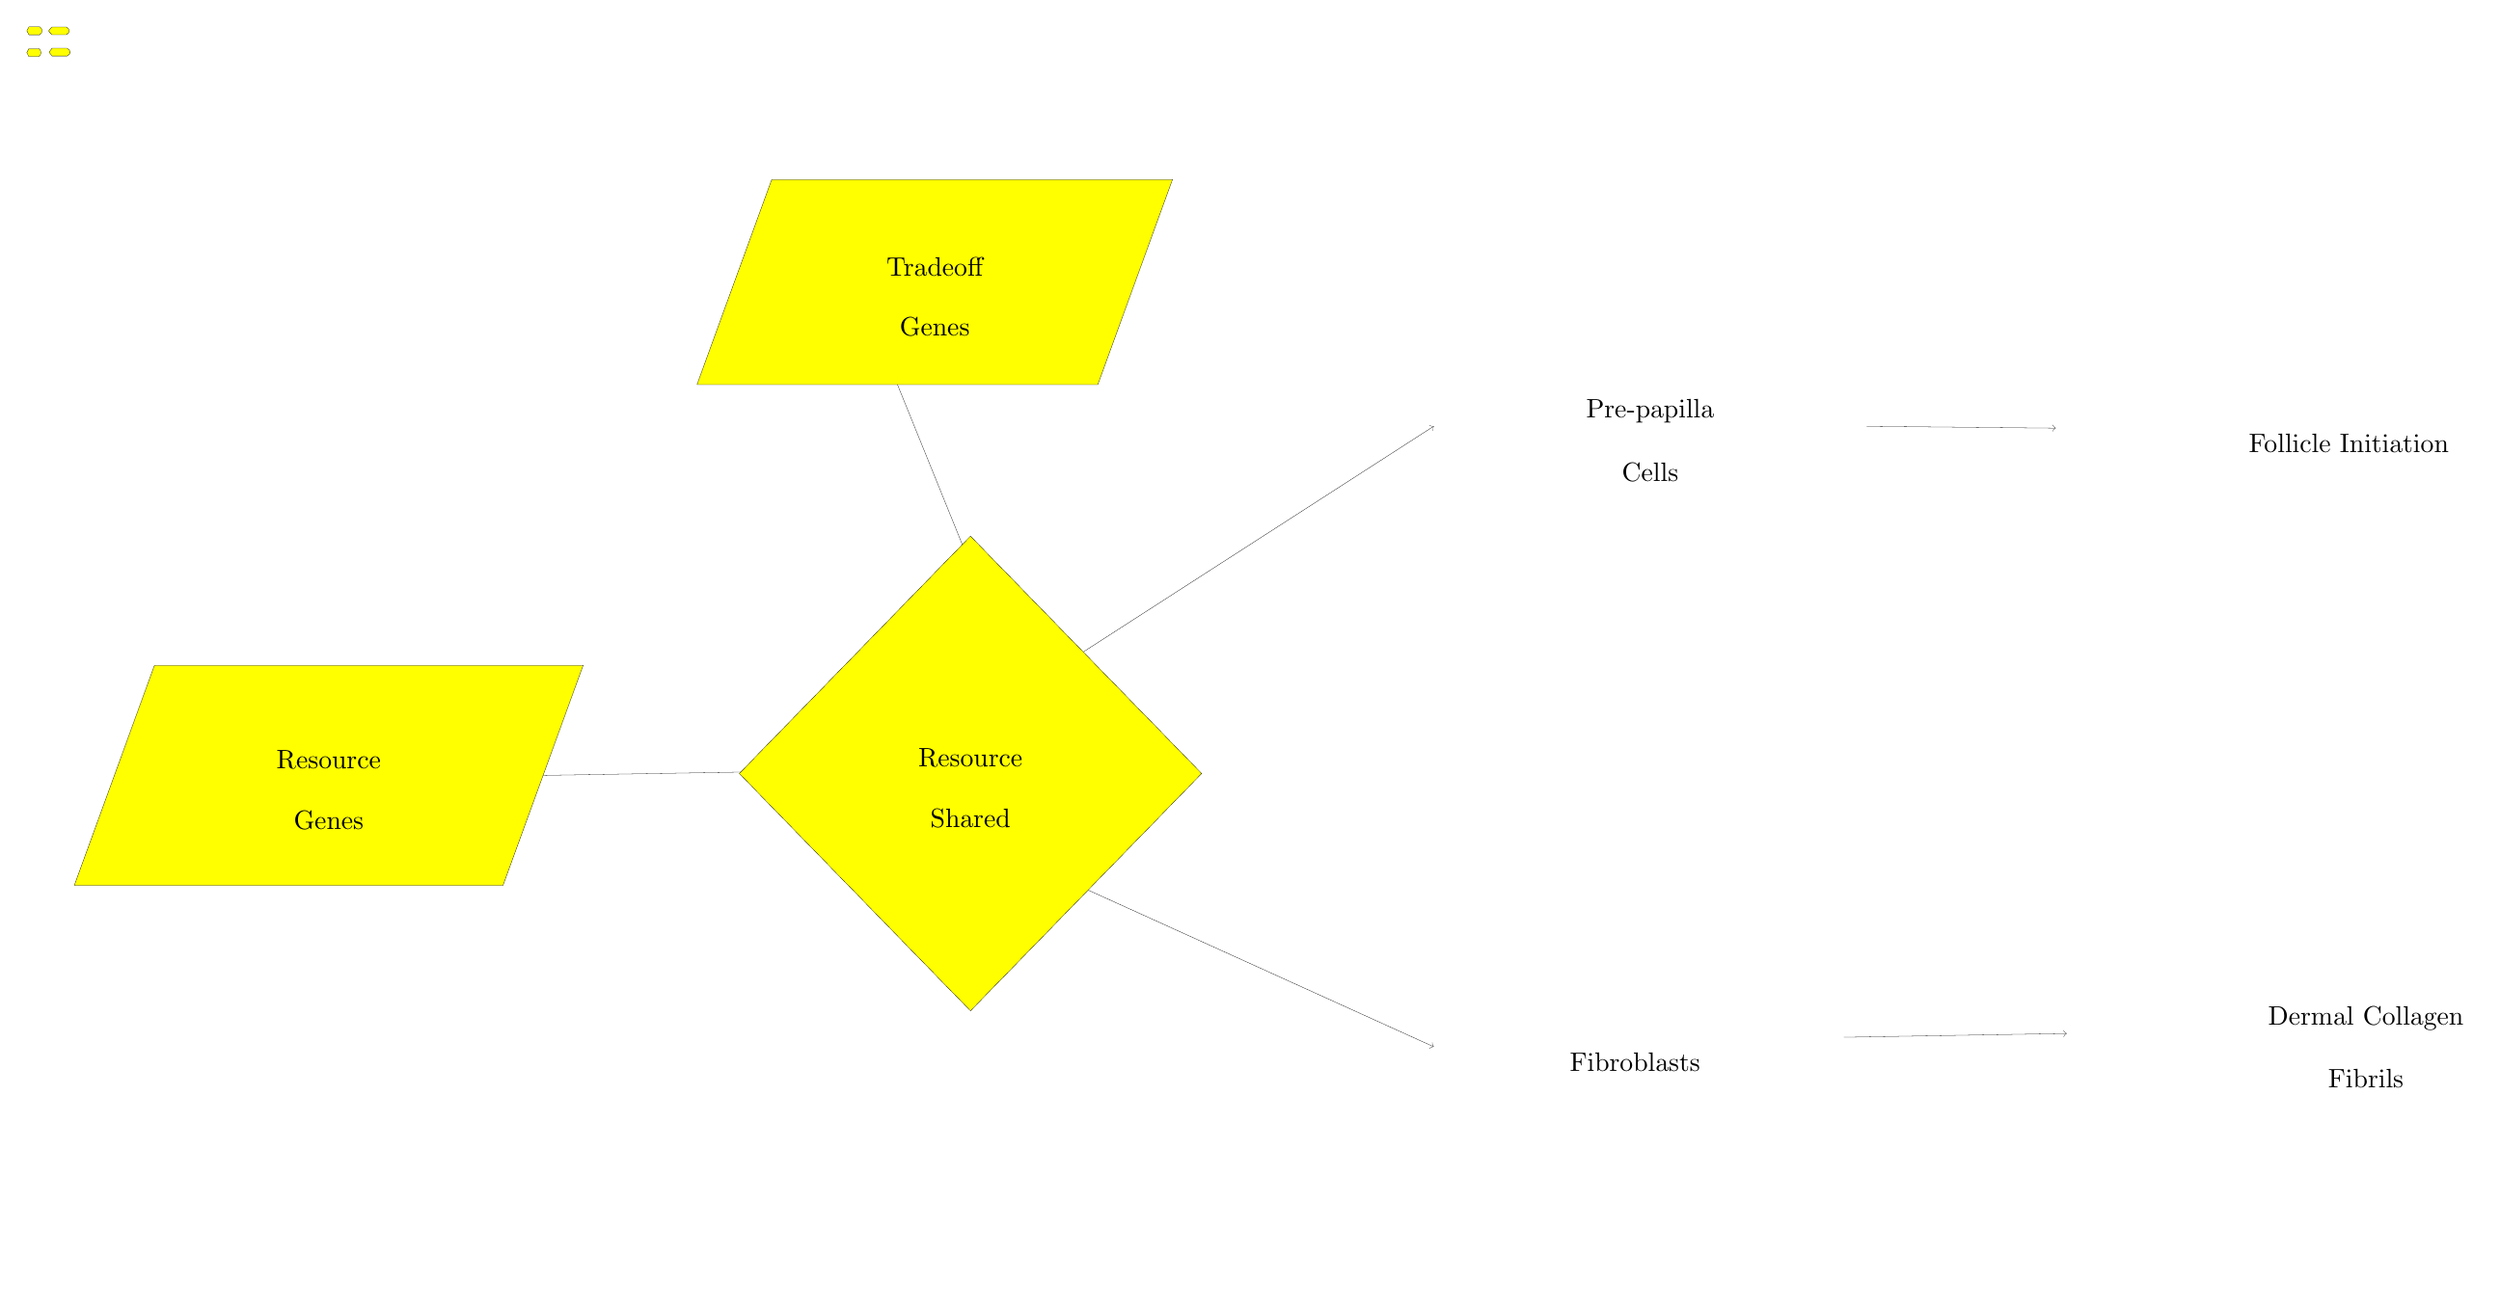
\begin{tikzpicture}
\pgftransformxscale{1.000000}
\pgftransformyscale{-1.000000}
\definecolor{dialinecolor}{rgb}{0.000000, 0.000000, 0.000000}
\pgfsetstrokecolor{dialinecolor}
\definecolor{dialinecolor}{rgb}{1.000000, 1.000000, 1.000000}
\pgfsetfillcolor{dialinecolor}
\pgfsetlinewidth{0.100000\du}
\pgfsetdash{}{0pt}
\pgfsetdash{}{0pt}
\pgfsetbuttcap
\pgfsetmiterjoin
\pgfsetlinewidth{0.100000\du}
\pgfsetbuttcap
\pgfsetmiterjoin
\pgfsetdash{}{0pt}
\definecolor{dialinecolor}{rgb}{1.000000, 1.000000, 0.000000}
\pgfsetfillcolor{dialinecolor}
\fill (13.050000\du,7.100000\du)--(15.650000\du,9.950000\du)--(13.050000\du,12.800000\du)--(10.450000\du,9.950000\du)--cycle;
\definecolor{dialinecolor}{rgb}{0.101961, 0.101961, 0.101961}
\pgfsetstrokecolor{dialinecolor}
\draw (13.050000\du,7.100000\du)--(15.650000\du,9.950000\du)--(13.050000\du,12.800000\du)--(10.450000\du,9.950000\du)--cycle;
\pgfsetbuttcap
\pgfsetmiterjoin
\pgfsetdash{}{0pt}
\definecolor{dialinecolor}{rgb}{0.101961, 0.101961, 0.101961}
\pgfsetstrokecolor{dialinecolor}
\draw (10.450000\du,9.950000\du)--(15.650000\du,9.950000\du);
\definecolor{dialinecolor}{rgb}{1.000000, 1.000000, 0.000000}
\pgfsetfillcolor{dialinecolor}
\fill (2.355514\du,8.550000\du)--(8.000000\du,8.550000\du)--(6.944486\du,11.450000\du)--(1.300000\du,11.450000\du)--cycle;
\pgfsetlinewidth{0.100000\du}
\pgfsetdash{}{0pt}
\pgfsetdash{}{0pt}
\pgfsetmiterjoin
\definecolor{dialinecolor}{rgb}{0.101961, 0.101961, 0.101961}
\pgfsetstrokecolor{dialinecolor}
\draw (2.355514\du,8.550000\du)--(8.000000\du,8.550000\du)--(6.944486\du,11.450000\du)--(1.300000\du,11.450000\du)--cycle;
% setfont left to latex
\definecolor{dialinecolor}{rgb}{0.101961, 0.101961, 0.101961}
\pgfsetstrokecolor{dialinecolor}
\node at (4.650000\du,9.795000\du){Resource};
% setfont left to latex
\definecolor{dialinecolor}{rgb}{0.101961, 0.101961, 0.101961}
\pgfsetstrokecolor{dialinecolor}
\node at (4.650000\du,10.595000\du){Genes};
% setfont left to latex
\definecolor{dialinecolor}{rgb}{0.101961, 0.101961, 0.101961}
\pgfsetstrokecolor{dialinecolor}
\node[anchor=west] at (4.650000\du,10.000000\du){};
% setfont left to latex
\definecolor{dialinecolor}{rgb}{0.101961, 0.101961, 0.101961}
\pgfsetstrokecolor{dialinecolor}
\node[anchor=west] at (4.650000\du,10.000000\du){   };
% setfont left to latex
\definecolor{dialinecolor}{rgb}{0.101961, 0.101961, 0.101961}
\pgfsetstrokecolor{dialinecolor}
\node[anchor=west] at (4.650000\du,10.000000\du){};
% setfont left to latex
\definecolor{dialinecolor}{rgb}{0.101961, 0.101961, 0.101961}
\pgfsetstrokecolor{dialinecolor}
\node[anchor=west] at (4.650000\du,10.000000\du){};
\definecolor{dialinecolor}{rgb}{1.000000, 1.000000, 0.000000}
\pgfsetfillcolor{dialinecolor}
\fill (10.482720\du,2.150000\du)--(15.759558\du,2.150000\du)--(14.776839\du,4.850000\du)--(9.500000\du,4.850000\du)--cycle;
\pgfsetlinewidth{0.100000\du}
\pgfsetdash{}{0pt}
\pgfsetdash{}{0pt}
\pgfsetmiterjoin
\definecolor{dialinecolor}{rgb}{0.101961, 0.101961, 0.101961}
\pgfsetstrokecolor{dialinecolor}
\draw (10.482720\du,2.150000\du)--(15.759558\du,2.150000\du)--(14.776839\du,4.850000\du)--(9.500000\du,4.850000\du)--cycle;
% setfont left to latex
\definecolor{dialinecolor}{rgb}{0.101961, 0.101961, 0.101961}
\pgfsetstrokecolor{dialinecolor}
\node at (12.629779\du,3.295000\du){Tradeoff};
% setfont left to latex
\definecolor{dialinecolor}{rgb}{0.101961, 0.101961, 0.101961}
\pgfsetstrokecolor{dialinecolor}
\node at (12.629779\du,4.095000\du){Genes};
% setfont left to latex
\definecolor{dialinecolor}{rgb}{0.101961, 0.101961, 0.101961}
\pgfsetstrokecolor{dialinecolor}
\node[anchor=west] at (12.629800\du,3.500000\du){};
% setfont left to latex
\definecolor{dialinecolor}{rgb}{0.101961, 0.101961, 0.101961}
\pgfsetstrokecolor{dialinecolor}
\node[anchor=west] at (12.629800\du,3.500000\du){};
% setfont left to latex
\definecolor{dialinecolor}{rgb}{0.101961, 0.101961, 0.101961}
\pgfsetstrokecolor{dialinecolor}
\node[anchor=west] at (12.629800\du,4.300000\du){};
% setfont left to latex
\definecolor{dialinecolor}{rgb}{0.101961, 0.101961, 0.101961}
\pgfsetstrokecolor{dialinecolor}
\node[anchor=west] at (12.629800\du,3.500000\du){};
% setfont left to latex
\definecolor{dialinecolor}{rgb}{0.101961, 0.101961, 0.101961}
\pgfsetstrokecolor{dialinecolor}
\node[anchor=west] at (12.629800\du,3.500000\du){};
% setfont left to latex
\definecolor{dialinecolor}{rgb}{0.101961, 0.101961, 0.101961}
\pgfsetstrokecolor{dialinecolor}
\node[anchor=west] at (12.629800\du,3.500000\du){};
% setfont left to latex
\definecolor{dialinecolor}{rgb}{0.101961, 0.101961, 0.101961}
\pgfsetstrokecolor{dialinecolor}
\node[anchor=west] at (12.629800\du,3.500000\du){};
% setfont left to latex
\definecolor{dialinecolor}{rgb}{0.101961, 0.101961, 0.101961}
\pgfsetstrokecolor{dialinecolor}
\node[anchor=west] at (13.050000\du,9.950000\du){};
% setfont left to latex
\definecolor{dialinecolor}{rgb}{0.101961, 0.101961, 0.101961}
\pgfsetstrokecolor{dialinecolor}
\node[anchor=west] at (13.050000\du,9.950000\du){};
% setfont left to latex
\definecolor{dialinecolor}{rgb}{0.101961, 0.101961, 0.101961}
\pgfsetstrokecolor{dialinecolor}
\node[anchor=west] at (13.050000\du,9.950000\du){};
% setfont left to latex
\definecolor{dialinecolor}{rgb}{0.101961, 0.101961, 0.101961}
\pgfsetstrokecolor{dialinecolor}
\node[anchor=west] at (13.050000\du,9.950000\du){};
% setfont left to latex
\definecolor{dialinecolor}{rgb}{0.101961, 0.101961, 0.101961}
\pgfsetstrokecolor{dialinecolor}
\node[anchor=west] at (5.300000\du,16.550000\du){};
% setfont left to latex
\definecolor{dialinecolor}{rgb}{0.101961, 0.101961, 0.101961}
\pgfsetstrokecolor{dialinecolor}
\node[anchor=west] at (13.050000\du,9.950000\du){};
% setfont left to latex
\definecolor{dialinecolor}{rgb}{0.101961, 0.101961, 0.101961}
\pgfsetstrokecolor{dialinecolor}
\node[anchor=west] at (13.050000\du,9.950000\du){};
% setfont left to latex
\definecolor{dialinecolor}{rgb}{0.101961, 0.101961, 0.101961}
\pgfsetstrokecolor{dialinecolor}
\node[anchor=west] at (13.050000\du,9.950000\du){};
% setfont left to latex
\definecolor{dialinecolor}{rgb}{0.101961, 0.101961, 0.101961}
\pgfsetstrokecolor{dialinecolor}
\node[anchor=west] at (13.050000\du,9.950000\du){};
% setfont left to latex
\definecolor{dialinecolor}{rgb}{0.101961, 0.101961, 0.101961}
\pgfsetstrokecolor{dialinecolor}
\node[anchor=west] at (13.050000\du,9.950000\du){};
% setfont left to latex
\definecolor{dialinecolor}{rgb}{0.101961, 0.101961, 0.101961}
\pgfsetstrokecolor{dialinecolor}
\node[anchor=west] at (11.750000\du,9.800000\du){Resource };
\pgfsetlinewidth{0.100000\du}
\pgfsetdash{}{0pt}
\pgfsetdash{}{0pt}
\pgfsetbuttcap
\pgfsetmiterjoin
\pgfsetlinewidth{0.100000\du}
\pgfsetbuttcap
\pgfsetmiterjoin
\pgfsetdash{}{0pt}
\definecolor{dialinecolor}{rgb}{1.000000, 1.000000, 0.000000}
\pgfsetfillcolor{dialinecolor}
\pgfpathmoveto{\pgfpoint{20.014286\du}{3.900000\du}}
\pgfpathlineto{\pgfpoint{24.085714\du}{3.900000\du}}
\pgfpathcurveto{\pgfpoint{24.696429\du}{4.500000\du}}{\pgfpoint{24.900000\du}{4.800000\du}}{\pgfpoint{24.900000\du}{5.400000\du}}
\pgfpathcurveto{\pgfpoint{24.900000\du}{6.000000\du}}{\pgfpoint{24.696429\du}{6.300000\du}}{\pgfpoint{24.085714\du}{6.900000\du}}
\pgfpathlineto{\pgfpoint{20.014286\du}{6.900000\du}}
\pgfpathlineto{\pgfpoint{19.200000\du}{5.400000\du}}
\pgfpathlineto{\pgfpoint{20.014286\du}{3.900000\du}}
\pgfusepath{fill}
\definecolor{dialinecolor}{rgb}{0.101961, 0.101961, 0.101961}
\pgfsetstrokecolor{dialinecolor}
\pgfpathmoveto{\pgfpoint{20.014286\du}{3.900000\du}}
\pgfpathlineto{\pgfpoint{24.085714\du}{3.900000\du}}
\pgfpathcurveto{\pgfpoint{24.696429\du}{4.500000\du}}{\pgfpoint{24.900000\du}{4.800000\du}}{\pgfpoint{24.900000\du}{5.400000\du}}
\pgfpathcurveto{\pgfpoint{24.900000\du}{6.000000\du}}{\pgfpoint{24.696429\du}{6.300000\du}}{\pgfpoint{24.085714\du}{6.900000\du}}
\pgfpathlineto{\pgfpoint{20.014286\du}{6.900000\du}}
\pgfpathlineto{\pgfpoint{19.200000\du}{5.400000\du}}
\pgfpathlineto{\pgfpoint{20.014286\du}{3.900000\du}}
\pgfusepath{stroke}
% setfont left to latex
\definecolor{dialinecolor}{rgb}{0.101961, 0.101961, 0.101961}
\pgfsetstrokecolor{dialinecolor}
\node at (22.050000\du,5.200000\du){Pre-papilla};
% setfont left to latex
\definecolor{dialinecolor}{rgb}{0.101961, 0.101961, 0.101961}
\pgfsetstrokecolor{dialinecolor}
\node at (22.050000\du,6.000000\du){Cells};
\pgfsetlinewidth{0.100000\du}
\pgfsetdash{}{0pt}
\pgfsetdash{}{0pt}
\pgfsetbuttcap
\pgfsetmiterjoin
\pgfsetlinewidth{0.100000\du}
\pgfsetbuttcap
\pgfsetmiterjoin
\pgfsetdash{}{0pt}
\definecolor{dialinecolor}{rgb}{1.000000, 1.000000, 0.000000}
\pgfsetfillcolor{dialinecolor}
\pgfpathmoveto{\pgfpoint{19.957143\du}{12.100000\du}}
\pgfpathlineto{\pgfpoint{23.742857\du}{12.100000\du}}
\pgfpathcurveto{\pgfpoint{24.310714\du}{12.690000\du}}{\pgfpoint{24.500000\du}{12.985000\du}}{\pgfpoint{24.500000\du}{13.575000\du}}
\pgfpathcurveto{\pgfpoint{24.500000\du}{14.165000\du}}{\pgfpoint{24.310714\du}{14.460000\du}}{\pgfpoint{23.742857\du}{15.050000\du}}
\pgfpathlineto{\pgfpoint{19.957143\du}{15.050000\du}}
\pgfpathlineto{\pgfpoint{19.200000\du}{13.575000\du}}
\pgfpathlineto{\pgfpoint{19.957143\du}{12.100000\du}}
\pgfusepath{fill}
\definecolor{dialinecolor}{rgb}{0.101961, 0.101961, 0.101961}
\pgfsetstrokecolor{dialinecolor}
\pgfpathmoveto{\pgfpoint{19.957143\du}{12.100000\du}}
\pgfpathlineto{\pgfpoint{23.742857\du}{12.100000\du}}
\pgfpathcurveto{\pgfpoint{24.310714\du}{12.690000\du}}{\pgfpoint{24.500000\du}{12.985000\du}}{\pgfpoint{24.500000\du}{13.575000\du}}
\pgfpathcurveto{\pgfpoint{24.500000\du}{14.165000\du}}{\pgfpoint{24.310714\du}{14.460000\du}}{\pgfpoint{23.742857\du}{15.050000\du}}
\pgfpathlineto{\pgfpoint{19.957143\du}{15.050000\du}}
\pgfpathlineto{\pgfpoint{19.200000\du}{13.575000\du}}
\pgfpathlineto{\pgfpoint{19.957143\du}{12.100000\du}}
\pgfusepath{stroke}
% setfont left to latex
\definecolor{dialinecolor}{rgb}{0.101961, 0.101961, 0.101961}
\pgfsetstrokecolor{dialinecolor}
\node at (21.850000\du,13.775000\du){Fibroblasts};
% setfont left to latex
\definecolor{dialinecolor}{rgb}{0.101961, 0.101961, 0.101961}
\pgfsetstrokecolor{dialinecolor}
\node[anchor=west] at (22.864300\du,5.400000\du){};
% setfont left to latex
\definecolor{dialinecolor}{rgb}{0.101961, 0.101961, 0.101961}
\pgfsetstrokecolor{dialinecolor}
\node[anchor=west] at (22.607100\du,13.575000\du){};
\pgfsetlinewidth{0.100000\du}
\pgfsetdash{}{0pt}
\pgfsetdash{}{0pt}
\pgfsetbuttcap
\pgfsetmiterjoin
\pgfsetlinewidth{0.100000\du}
\pgfsetbuttcap
\pgfsetmiterjoin
\pgfsetdash{}{0pt}
\definecolor{dialinecolor}{rgb}{1.000000, 1.000000, 0.000000}
\pgfsetfillcolor{dialinecolor}
\pgfpathmoveto{\pgfpoint{28.492500\du}{4.000000\du}}
\pgfpathlineto{\pgfpoint{34.007500\du}{4.000000\du}}
\pgfpathcurveto{\pgfpoint{34.834750\du}{4.570000\du}}{\pgfpoint{35.110500\du}{4.855000\du}}{\pgfpoint{35.110500\du}{5.425000\du}}
\pgfpathcurveto{\pgfpoint{35.110500\du}{5.995000\du}}{\pgfpoint{34.834750\du}{6.280000\du}}{\pgfpoint{34.007500\du}{6.850000\du}}
\pgfpathlineto{\pgfpoint{28.492500\du}{6.850000\du}}
\pgfpathlineto{\pgfpoint{27.389500\du}{5.425000\du}}
\pgfpathlineto{\pgfpoint{28.492500\du}{4.000000\du}}
\pgfusepath{fill}
\definecolor{dialinecolor}{rgb}{0.101961, 0.101961, 0.101961}
\pgfsetstrokecolor{dialinecolor}
\pgfpathmoveto{\pgfpoint{28.492500\du}{4.000000\du}}
\pgfpathlineto{\pgfpoint{34.007500\du}{4.000000\du}}
\pgfpathcurveto{\pgfpoint{34.834750\du}{4.570000\du}}{\pgfpoint{35.110500\du}{4.855000\du}}{\pgfpoint{35.110500\du}{5.425000\du}}
\pgfpathcurveto{\pgfpoint{35.110500\du}{5.995000\du}}{\pgfpoint{34.834750\du}{6.280000\du}}{\pgfpoint{34.007500\du}{6.850000\du}}
\pgfpathlineto{\pgfpoint{28.492500\du}{6.850000\du}}
\pgfpathlineto{\pgfpoint{27.389500\du}{5.425000\du}}
\pgfpathlineto{\pgfpoint{28.492500\du}{4.000000\du}}
\pgfusepath{stroke}
% setfont left to latex
\definecolor{dialinecolor}{rgb}{0.101961, 0.101961, 0.101961}
\pgfsetstrokecolor{dialinecolor}
\node at (31.250000\du,5.625000\du){Follicle Initiation};
\pgfsetlinewidth{0.100000\du}
\pgfsetdash{}{0pt}
\pgfsetdash{}{0pt}
\pgfsetbuttcap
\pgfsetmiterjoin
\pgfsetlinewidth{0.100000\du}
\pgfsetbuttcap
\pgfsetmiterjoin
\pgfsetdash{}{0pt}
\definecolor{dialinecolor}{rgb}{1.000000, 1.000000, 0.000000}
\pgfsetfillcolor{dialinecolor}
\pgfpathmoveto{\pgfpoint{28.660000\du}{11.950000\du}}
\pgfpathlineto{\pgfpoint{34.290000\du}{11.950000\du}}
\pgfpathcurveto{\pgfpoint{35.134500\du}{12.530000\du}}{\pgfpoint{35.416000\du}{12.820000\du}}{\pgfpoint{35.416000\du}{13.400000\du}}
\pgfpathcurveto{\pgfpoint{35.416000\du}{13.980000\du}}{\pgfpoint{35.134500\du}{14.270000\du}}{\pgfpoint{34.290000\du}{14.850000\du}}
\pgfpathlineto{\pgfpoint{28.660000\du}{14.850000\du}}
\pgfpathlineto{\pgfpoint{27.534000\du}{13.400000\du}}
\pgfpathlineto{\pgfpoint{28.660000\du}{11.950000\du}}
\pgfusepath{fill}
\definecolor{dialinecolor}{rgb}{0.101961, 0.101961, 0.101961}
\pgfsetstrokecolor{dialinecolor}
\pgfpathmoveto{\pgfpoint{28.660000\du}{11.950000\du}}
\pgfpathlineto{\pgfpoint{34.290000\du}{11.950000\du}}
\pgfpathcurveto{\pgfpoint{35.134500\du}{12.530000\du}}{\pgfpoint{35.416000\du}{12.820000\du}}{\pgfpoint{35.416000\du}{13.400000\du}}
\pgfpathcurveto{\pgfpoint{35.416000\du}{13.980000\du}}{\pgfpoint{35.134500\du}{14.270000\du}}{\pgfpoint{34.290000\du}{14.850000\du}}
\pgfpathlineto{\pgfpoint{28.660000\du}{14.850000\du}}
\pgfpathlineto{\pgfpoint{27.534000\du}{13.400000\du}}
\pgfpathlineto{\pgfpoint{28.660000\du}{11.950000\du}}
\pgfusepath{stroke}
% setfont left to latex
\definecolor{dialinecolor}{rgb}{0.101961, 0.101961, 0.101961}
\pgfsetstrokecolor{dialinecolor}
\node at (31.475000\du,13.200000\du){Dermal Collagen};
% setfont left to latex
\definecolor{dialinecolor}{rgb}{0.101961, 0.101961, 0.101961}
\pgfsetstrokecolor{dialinecolor}
\node at (31.475000\du,14.000000\du){Fibrils};
% setfont left to latex
\definecolor{dialinecolor}{rgb}{0.101961, 0.101961, 0.101961}
\pgfsetstrokecolor{dialinecolor}
\node[anchor=west] at (32.353000\du,5.425000\du){};
% setfont left to latex
\definecolor{dialinecolor}{rgb}{0.101961, 0.101961, 0.101961}
\pgfsetstrokecolor{dialinecolor}
\node[anchor=west] at (32.601000\du,13.400000\du){};
\pgfsetlinewidth{0.100000\du}
\pgfsetdash{}{0pt}
\pgfsetdash{}{0pt}
\pgfsetbuttcap
{
\definecolor{dialinecolor}{rgb}{0.101961, 0.101961, 0.101961}
\pgfsetfillcolor{dialinecolor}
% was here!!!
\pgfsetarrowsend{to}
\definecolor{dialinecolor}{rgb}{0.101961, 0.101961, 0.101961}
\pgfsetstrokecolor{dialinecolor}
\draw (7.472240\du,10.000000\du)--(10.450000\du,9.950000\du);
}
\pgfsetlinewidth{0.100000\du}
\pgfsetdash{}{0pt}
\pgfsetdash{}{0pt}
\pgfsetbuttcap
{
\definecolor{dialinecolor}{rgb}{0.101961, 0.101961, 0.101961}
\pgfsetfillcolor{dialinecolor}
% was here!!!
\pgfsetarrowsend{to}
\definecolor{dialinecolor}{rgb}{0.101961, 0.101961, 0.101961}
\pgfsetstrokecolor{dialinecolor}
\draw (12.138400\du,4.850000\du)--(13.050000\du,7.100000\du);
}
\pgfsetlinewidth{0.100000\du}
\pgfsetdash{}{0pt}
\pgfsetdash{}{0pt}
\pgfsetbuttcap
{
\definecolor{dialinecolor}{rgb}{0.101961, 0.101961, 0.101961}
\pgfsetfillcolor{dialinecolor}
% was here!!!
\pgfsetarrowsend{to}
\definecolor{dialinecolor}{rgb}{0.101961, 0.101961, 0.101961}
\pgfsetstrokecolor{dialinecolor}
\draw (14.350000\du,8.525000\du)--(19.200000\du,5.400000\du);
}
\pgfsetlinewidth{0.100000\du}
\pgfsetdash{}{0pt}
\pgfsetdash{}{0pt}
\pgfsetbuttcap
{
\definecolor{dialinecolor}{rgb}{0.101961, 0.101961, 0.101961}
\pgfsetfillcolor{dialinecolor}
% was here!!!
\pgfsetarrowsend{to}
\definecolor{dialinecolor}{rgb}{0.101961, 0.101961, 0.101961}
\pgfsetstrokecolor{dialinecolor}
\draw (14.350000\du,11.375000\du)--(19.200000\du,13.575000\du);
}
\pgfsetlinewidth{0.100000\du}
\pgfsetdash{}{0pt}
\pgfsetdash{}{0pt}
\pgfsetbuttcap
{
\definecolor{dialinecolor}{rgb}{0.101961, 0.101961, 0.101961}
\pgfsetfillcolor{dialinecolor}
% was here!!!
\pgfsetarrowsend{to}
\definecolor{dialinecolor}{rgb}{0.101961, 0.101961, 0.101961}
\pgfsetstrokecolor{dialinecolor}
\draw (24.900000\du,5.400000\du)--(27.389500\du,5.425000\du);
}
\pgfsetlinewidth{0.100000\du}
\pgfsetdash{}{0pt}
\pgfsetdash{}{0pt}
\pgfsetbuttcap
{
\definecolor{dialinecolor}{rgb}{0.101961, 0.101961, 0.101961}
\pgfsetfillcolor{dialinecolor}
% was here!!!
\pgfsetarrowsend{to}
\definecolor{dialinecolor}{rgb}{0.101961, 0.101961, 0.101961}
\pgfsetstrokecolor{dialinecolor}
\draw (24.600000\du,13.450000\du)--(27.534000\du,13.400000\du);
}
\definecolor{dialinecolor}{rgb}{1.000000, 1.000000, 0.000000}
\pgfsetfillcolor{dialinecolor}
\fill (13.100000\du,6.848080\du)--(16.143904\du,9.975000\du)--(13.100000\du,13.101920\du)--(10.056096\du,9.975000\du)--cycle;
\pgfsetlinewidth{0.100000\du}
\pgfsetdash{}{0pt}
\pgfsetdash{}{0pt}
\pgfsetmiterjoin
\definecolor{dialinecolor}{rgb}{0.101961, 0.101961, 0.101961}
\pgfsetstrokecolor{dialinecolor}
\draw (13.100000\du,6.848080\du)--(16.143904\du,9.975000\du)--(13.100000\du,13.101920\du)--(10.056096\du,9.975000\du)--cycle;
% setfont left to latex
\definecolor{dialinecolor}{rgb}{0.101961, 0.101961, 0.101961}
\pgfsetstrokecolor{dialinecolor}
\node at (13.100000\du,9.770000\du){Resource};
% setfont left to latex
\definecolor{dialinecolor}{rgb}{0.101961, 0.101961, 0.101961}
\pgfsetstrokecolor{dialinecolor}
\node at (13.100000\du,10.570000\du){Shared};
% setfont left to latex
\definecolor{dialinecolor}{rgb}{0.101961, 0.101961, 0.101961}
\pgfsetstrokecolor{dialinecolor}
\node[anchor=west] at (13.100000\du,9.975000\du){};
\end{tikzpicture}
  \caption{Diagram of the postulated tradeoff relationship between pre-papilla cell differentiation and fibroblast differerentiation}
\end{figure}
\end{landscape}
%\end{document}



If there is lots of variation between sheep in the {\em tradeoff genes} and not much genetic variation in the {\em resource genes}, then the shared resource will be limiting, and the numbers of differentiating pre-papilla cells and fibroblasts will be negatively related, and this will result in a negtive correlation between numbers of initiating follicles and amount of dermal collagen. This would seem to be the case in the present data. If there is lots of genetic variation in the resource genes, so that the quantity of resource itself varies, then the above correlation may be positive, reflecting a situation where 'more of everything' is possible. 

\subsection{Pre-papilla cell number and follicle number and fibre diameter}
A large number of pre-papilla cells does not necessarily lead to a lot of follicles. They may form larger follicles ( more papilla cells per follicle) and thus grow larger fibres ( hight fibre diameter).
So if we believe the tradeoff relationship between fibroblasts and pre-papille cells discussed above, we should examine the relation between CST measurement  and number of pre-papilla cells. We cant measure number of pre-papilla cells, but we can estimate it by
\begin{displaymath}
N = N_{p} \pi \left[\frac{D_{p}}{2}\right]^2 + N_{s} \pi \left[\frac{D_{s}}{2}\right]^2
\end{displaymath}
which is a weighted sum of $N_{p}$ and $N_{s}$, the weights being fibre cross sectional areas. N should be proportional to the final number of papilla cells after follicle formation is complete.

What we know from present data is that there are medium correlations of CST with both Fn and Ds. The correlation with Fn is negative and this supports the idea that low collagen means more pre-papilla cells. The correlation with Ds is positive, so this does not support the idea that low collagen means bigger fibres. Diameter determination is more complex than just the number of available pre-papilla cells. 

So the idea that we could use N above as an index of number of papilla cells is probably flawed. We shall not proceed with N. We just note that determining pre-papilla cell number is not the final word on determining follicle number and fibre diameter jointly.

\subsection{Collagen and follicle curvature, follicle unevenness, and SD of fibre diameter}
There is a serious  question arising from the relation between CST and follicle curvature (Figure~\ref{fig:CSTFc}. We do not understand why a high CST is always a high follicle curvature, but a low CST can be any curvature from 1 to 7. 

The fact that in some sheep follicles curve when the collagen is soft or minimal implies that there is a secondary cause of follicle curvature which is only expressed when CST is low. We do not know what this secondary cause is. 

\subsection{Collagen and wrinkle}
This is really a topic requiring further research. We only have a relationship between SkinType and collagen. The "tight" Skintype had higher CST and lower Compressibility, than the other Skintypes. The "tight" SkinType is wrinkled. Therefore, indirctly, wrinkled sheep have more collagen. 

We have no data relating compressed skin thickness measurements to various degrees of wrinkle, such as are described by wrinkle scores on the neck and side regions of sheep. 

We need to know where the collagen is in the skin in relation to wrinkles, and both the amount and type ( hard or soft) of collagen. That work in proceeding. 

What we can say here is that one of the predisposing factors in the skin leading to wrinkle formation is the presence of large amounts of collagen. Another predisposing factor is excess growth expansion of the dermis, relative to the subdermal layers. This latter factor is investigated in Jackson and Watts(2018)~\cite{jack:18}, where it is shown that the  proliferation of Sd follicles in the Merino foetus at around 100 days  will cause an excess dermal expansion of 20 to 30 percent, over and above normal growth of all the skin layers. This is sufficient to form a skin fold. Both predisposing factors must be present for wrinkles to form.


\clearpage
\begin{thebibliography}{99}

\bibitem{bogo:40}
 Bogolyubsky S.N. (1940) cited by Fraser A.S and Short B.F. (1960) The Biology of the Fleece. Animal Research Laboratories Technical Paper No 3. CSIRO Melbourne 1960.

\bibitem{brow:68}
Brown, G.H., and Turner, Helen Newton. (1968) Response to selection in Australian Merino sheep. II. Estimates of phenotypic and genetic parameters for some production traits in Merino ewes and an analysis of the possible effects of selection on them. Aust. J. Agric. Res. 19:303-22

\bibitem{cart:43}
Carter H.B. (1943) Studies in the biology of the skin and fleece of sheep. 1. The development and general histology of the follicle group in the skin of the Merino. 2. The use of tanned sheepskin in the study of follicle population density. 3. Notes on the arrangement, nomenclature, and variation of skin folds and wrinkles in the Merino. C.S.I.R. Bulletin No 164, Melbourne, 1943

\bibitem{fras:60}
Fraser A.S and Short B.F. (1960) The Biology of the Fleece. Animal Research Laboratories Technical Paper No 3. CSIRO Melbourne 1960.

\bibitem{gord:08}
Gordon-Thompson, C., Botto, S.A., Cam, G.R., and Moore, G.P.H. (2008) Notch pathway gene expression and wool follicle cell fates. Aust. J. Exp. Agric. 48(5) 648-656

\bibitem{jack:75}
Jackson, N., Nay, T, and Turner, Helen Newton (1975) Response to selection in Australian Merino sheep. VII Phenotypic and genetic parameters for some wool follicle characteristics and their correlation with wool and body traits. Aust. J. Agric. Res. 26:937-57

\bibitem{jack:15}
Jackson, N. (2015) Genetic relationship betweeen skin and wool traits in Merino sheep. Incomplete manuscript.

\bibitem{jack:17}
Jackson, N. (2017) Genetics of primary and secondary fibre diameters and densities in Merino sheep. URL https://github.com/nevillejackson/atavistic-sheep/mev-rewrite/supplementary/genetic-parameters/psparam.pdf

\bibitem{jack:17a}
Jackson, N. (2017) Genetic relationship between skin and wool traits in Merino sheep. Part I Responses to selection ans estimates of genetic parameters. URL https://github.com/nevillejackson/Fleece-genetics/tree/master/skinandfleeceparameters/ab3220/skinwool1.pdf

\bibitem{jack:18}
Jackson, N. and Watts, J.E. (2018) Does follicle development affect the spatial layout of sheep skin? URL https://github.com/nevillejackson/Fleece-biology/tree/master/skinspace/skinspace.pdf

\bibitem{jack:90}
Jackson, N., Maddocks, I.G., Lax, J., Moore, G.P.M. and Watts, J.E. (1990) Merino Evolution, Skin Characteristics, and Fleece Quality. URL https://github.com/nevillejackson/atavistic-sheep/mev/evol.pdf 

\bibitem{jack:17b}
Jackson, N. and Watts, J.E. (2017) What is known about the genetics of wrinkle score in Merino sheep? URL https://github.com/nevillejackson/Fleece-genetics/wrinkle/wrinkle.pdf

\bibitem{knig:93}
Knight, K.R., Lepore, D.A., Horne, R.S., Ritz, M., Kumta, S. and O'Brian, B.M. (1993) Collagen content of uninjured skin and scar tissue in foetal and adult sheep. Int. J. Exp. Pathol. 74(6):583-591

\bibitem{madd:88}
Maddocks, I.G. and Jackson, N. (1988) Structural studies of sheep, cattle, and goat skin. CSIRO, Division of Aimal Production, Sydney.

\bibitem{ment:80}
Menton, D.N. and Hess, R.A. (1980) The ultrastructure of collagen in the dermis of tight-skin (Tsk) mutant mice. The Journal of Investigative Dermatology 74:139-147

\bibitem{mitc:84}
Mitchell, T.W. et al (1984) Wool Technology and Sheep Breeding, No IV, 200-206

\bibitem{moor:89}
Moore G.P.M., Jackson, N., and Lax, J. (1989) Evidence of a unique developmental mechanism specifying bot wool follicle density and fibre size in sheep selected for single skin and fleece characters. Genet. Res. Camb. 53:57-62

\bibitem{moor:98}
Moore, G.P.M., Jackson, N., Isaacs, K., and Brown, G (1998) J. Theoretical Biology 191:87-94

\bibitem{nay:66}
Nay, T. (1966) Wool follicle arrangement and vascular pattern in the Australian Merino. Aust. J. Agric. Res. 17:797-805

\bibitem{rprog:13}
R Core Team (2013). R: A language and environment for statistical
  computing. R Foundation for Statistical Computing, Vienna, Austria.
  ISBN 3-900051-07-0, URL http://www.R-project.org/.

\bibitem{ryde:68}
Ryder, M.L. and Stevenson, S.K.(1968) Wool Growth. Academic Press, London.


\bibitem{turn:56} 
Turner, Helen Newton (1956) Anim. Breed. Abstr. 24:87-118

\bibitem{turn:58}
Turner, Helen Newton(1958) Aust. J. Agric. Res. 9:521-52

\bibitem{turn:53}
Turner, Helen Newton, Hayman, R.H., Riches, J.H., Roberts, N.F., and Wilson, L.T. (1953) Physical definition of sheep and their fleece for breeding and husbandry studies: with particular reference to Merino sheep. CSIRO Div. Anim. Hlth. Prod. Div. Rept. No. 4 (Ser SW-2 mimeo)

\bibitem{turn:70}
Turner, Helen Newton, Brooker M.G. and Dolling, C.H.S (1970) Response to selection in Australian Merino sheep. III Single character selection for high and low values of wool weight and its components. Aust.J.Agric.Res. 21:955-84

\bibitem{watt:17}
Watts, J.E., Jackson, N., and Ferguson, K.A. (2017) Improvements in fleece weight weight and wool quality of Merino sheep selected visually for high fibre density and length. URL https://github.com/nevillejackson/SRS-Merino/Paper\_2\_Revised\_10\_November\_2017.docx 

\bibitem{xavi:03}
Xavier, S.P., Gordon-Thomson, C. Wynn, P.C., McCullagh, P., Thomson, P.C., Tomkins, L., Mason, R.S., and Moore, G.P.M.(2003) Evidence that Notch and Delta expressions have a role in dermal condensate aggregation during wool follicle initiation. Experimental Dermatology, 22:656-681

\end{thebibliography}
\end{document}
